\documentclass{article}
\usepackage{bchow}

%font
\setmainfont{KpLight}
\setsansfont{CMU Bright}[Scale=MatchLowercase]
\setmonofont{KpMono}
\setmathfont{KpMath-Light.otf}[math-style=ISO,bold-style=TeX,StylisticSet={1,3,4},CharacterVariant={2,3,6}]

\renewcommand{\familydefault}{\rmdefault}

%image path
\graphicspath{{./figure/}}

\begin{document}
	\title{{ECOS3031}\\{\normalsize{Heterodox Perspectives on Macroeconomics -- Notes}}}
	\author{Brendan Chow}
	\abstract{Based on the lecture notes by A/Prof Graham White}
	\affiliation{
	Student at the University of Sydney\\
	\href{https://xagill.com/}{Website}\\
	\href{https://www.linkedin.com/in/brendanchow/}{LinkedIn}\\
	\href{https://github.com/ARocketdog}{GitHub}\\
	}
	\emailAdd{brendanchow@xagill.com}
	\maketitle
	\newpage
	\pagestyle{fancynotes}
	\pagenumbering{arabic}
%start document
\section{Background: Two Traditions in the Theory of Output}
\subsection{Introduction}
	\begin{itemize}
		\item Important in understanding the nature of macro orthodoxy
		\item But also the significance of criticism of orthodoxy
		\item Story of where we are now really revolves around long running tension between two grand traditions in the theory of output
		\begin{itemize}
			\item a dominant tradition emerging from the late 19th century
			\item a dissenting tradition associated most with the work of Keynes
		\end{itemize}
	\end{itemize}
\subsection{Two Traditions in the Theory of Output}
	\begin{itemize}
		\item Since the mid 19th century - two opposing views about the forces which govern the aggregate level (rate of growth) of output (activity)
		\item These differ as to whether it is demand or output (and output capacity) which is the independent variable
		\item Dominant view over 200 years that demand does not provide an independent long-run constraint on output
		\item Alternative position in Keynes (1936) and Kalecki (1935) (and sporadically beforehand e.g. Marx) - and a rich undercurrent of dissent since Keynes to the present
		\item Demand provides an independent constraint on the level (rate of growth) of output in the long-run, no less than the short-run
		\item With a given technique of production and thus a given employment-output link, these two different views \( \Rightarrow \) opposing views about what governs employment and unemployment
		\item The dominant view \( \Rightarrow \) full utilisation of resources is the limit on employment
		\item If there is a market based mechanism to bring the economy to that limit \( \Rightarrow \) little long-run role for demand-management policy as a means of securing full-employment
		\item The case for macro demand management seen to turns on the efficacy of the market ``mechanism''
		\item At a fundamental theoretical level the debate is over the long-run relation between saving and investment
		\item Yet, by the 1970's the notion that the Keynesian position was relevant even for the short-run was under challenge from ``rational expectations'' and what was to become ``new classical macroeconomics''
	\end{itemize}
\subsection{Wicksell and the Premises of Traditional Theory}
	\begin{itemize}
		\item Wicksell's analysis seen by many as one of the most important (before and after Keynes) in providing foundations for the traditional/dominant theory of output
		\item By means of the theory of the rate of interest
		\item Wicksell's analysis was a leading example of ``marginalist theory'' dominant from the 1870's
	\end{itemize}
	\subsubsection{Marginalism}
	\begin{itemize}
		\item Fundamental role of scarcity in the explanation of prices, distribution and outputs 
		\item Prices are the solution to the allocation problem generated by the existence of ``scarce'' resources
		\item Equilibrium prices permit the allocation problem to be solved consistent with profit-max. objectives of producers and utility-max objectives of consumers
		\item ``Prices'' here included the rates of payment to so-called ``factors of production''
		\item Equilibrium rates of payment balanced demands and supplie\textbf{s} of factors, including labour
		\item Early generations of marginalist theory located the foundation of the theory of the rate of interest within this framework
		\item In the ``long-run'' as the equilibrium rate of payment for a specific factor of production, \textit{capital}
		\item As an explanation for the rate of interest this theory has held sway within standard macroeconomics to the present day
		\item Better known form: \textit{the real rate of interest ultimately reflects the balance between the demand and supply of saving}, where the demand for saving can be interpreted as the demand for investment
		\item Nonetheless, the analytics foundations lie in the theory of capital: \textit{the real rate of interest ultimately reflects the demand and supply of capital (as flows)}
	\end{itemize}
	\subsubsection{Marginalism and capital}
	\begin{itemize}
		\item Representation of capital as a ``factor of production'' akin to ``primary factors''
		\item Has played and continues to play a fundamental role in orthodox economic theory - specifically in the theory of distribution
		\item Two aspects to this:
		\begin{enumerate}[(i)]
			\item explaining the return to capital in a manner analogous to the explanation of rates of return on labour and land;
			\item defining an ``endowment'' of capital analogous to the endowments of labour and land \( \Rightarrow \) consistent with the notion of economics being primarily concerned with an allocation problem
		\end{enumerate}
		\item Two different approaches to defining this endowment - Walras and Wicksell
		\item For both there would exist an ``endowment'' of capital analogous to the endowment of labour and land (i.e. primary factors)
		\item Both approaches suffered from fundamental theoretical difficulties - brought to light by 20th century debates
		\item Arguably modern macro theory's position on the rate of interest as the mechanism bringing investment into line with saving owes more to Wicksell's approach
		\item Determining the rate of return on capital analogously to the explanation of the real wage for labour and rent on land required a view of the demand for capital analogous to demand for primary factors
		\item \( \Rightarrow \) being able to link propositions about marginal returns to the factor to demand for the factor - analogous to the case of land and labour 
		\item Required application of a ``homogeneity proposition''
		\item  \textit{viz.}, that different methods of producing commodities involving different capital goods could be thought of as embodying different amounts of a homogeneous ``capital''
		\item \( \Rightarrow \) could represent different techniques as different ratios of labour to capital for example, i.e. representing different proportions between different `factors of production' 
		\item For Wicksell capital represents ``saved-up'' labour and land
		\item \( \Rightarrow \) resources ``set free'' by abstinence from consumption and available for embodiment in capital goods
		\item Different capital goods could be thought of as embodying different amounts of a homogeneous capital, where the latter represents different amounts of saved up land and saved-up labour
		\item A means of treating produced capital goods - i.e. a heterogeneous collection of produced commodities  - as homogneous
		\item And in turn \( \Rightarrow \) different methods of production as different amounts of a labour and land relative to homogeneous ``capital
		\item Could then speak of ``productivity of capital at the margin''
		\item And of substitution between capital and primary factors in response to relative factor prices
		\item \( \Rightarrow \) ``demand for capital'' inversely related to its rate of return based on marginal productivity
		\item Theoretically, the basis of demand for investment as a function of the return to capital 
		\item To facilitate the discussion, assume that over time the rental rate on capital should reflect the ``rate of interest'' plus a margin for risk
		\item The rate of interest represents the opportunity cost of employing resources in the production of capital goods
		\item Thinking of the \( I\:(r_k) \) relation as representing long-period levels of investment \( \Rightarrow \) represents also a demand for investment as a function of the rate of interest
		\item The marginal productivity theory applied to capital \( \Rightarrow \) the foundation for the orthodox explanation of investment as a decreasing function of the rate of interest
		\item Other elements of orthodox theory would eventually link saving to the rate of interest
		\item \( \Rightarrow \) a saving function reflecting the rate of ``time-preference''
		\begin{figure}[H]
			\centering
			\begin{tikzpicture}[scale=0.55]
			\draw[thick] (0,9) node[left]{\( i \)} -- (0,0) -- (9,0) node[below]{\( S, I \)};
			\draw [thick] (1,7.5) -- (8,1);
			\draw [thick] (1,1.5) -- (7.5,8) node[right]{\( S=f(i) \)};
			\end{tikzpicture}
		\end{figure}
		\item Combined with a ``supply'' of resources set free by saving \( \Rightarrow \) a demand and supply explanation of the equilibrium return to capital 
		\item Analogous to that for primary factors
		\item BUT -- what of the rate of interest?
		\item Typically observed as a ``monetary phenomenon''
		\item And subject to influence by monetary policy?
		\item \( \Rightarrow \) significance of Wicksell's monetary theory
		\item  ``This theory constitutes perhaps the most important pre-Keynesian attempt to ground by means of a systematic analysis of the money loan market (the market in which the rate of interest is actually observed) the marginalist concept of interest as the supply-and-demand determined price of the productive factor `capital' (Garegnani, 1978)''
		\item For Wicksell, although interest appears as a monetary phenomenon, it is ultimately dictated by ``real forces'' (productivity of capital and thrift)
		\item In Wicksell's view, even with saving taking a monetary form, explanation of the rate of interest in terms of real forces would still hold good
		\item Also, to the extent that the rate of interest is regulated by the equilibrium return to capital \( \Rightarrow \) the rate of interest could be seen as reflecting the ``scarcity of capital'' and as a reward for ``waiting''
		\item  Wicksell's answers bound up in part with a defence of the `quantity theory of money'
		\item \( \Rightarrow \) the mechanics by which changes in the quantity of money would ultimately impact on the price level
		\item And with the links between the rate of interest and the price level
		\item Primary cause of price fluctuations seen to be divergence between actual money or market rate of interest on loans from the ``natural rate'' which balances demand and supply of saving and reflects the scarcity of capital
		\item  Wicksell: absent a banking system, with loans between individuals, the ``loan'' rate should reflect demand and supply of saving
		\item Hence:
		\begin{quote}
			``an immediate connection between the loan rate and the real capital rate \ldots [c]hanges in the loan rate would take place simultaneously and uniformly with changes in the real rate'' (Pivetti, New Plagrave)
		\end{quote}	
		\item  Existence of a banking system breaks the connection between these two rates to the extent that bank lending is determined independently of the flow of money saving
		\item \textbf{BUT} a longer-run connection is maintained via fluctuations in the price level
		\item \textbf{AND} the latter is primarily due to to differences between these market and natural rates rates
		With fully flexible real wages, labour market tends to full-employment
		\item \( \Rightarrow \) divergences between market and natural interest rates \( \Rightarrow \) (via saving-investment gap) either price inflation or price deflation
		\item  To the extent that monetary equilibrium requires stability of the price level \( \Rightarrow \) market rate must come into line with the natural rate
		\item For Wicksell, problem is banking system being able to adjust the market rate to variations in the natural rate resulting from changes in capital productivity and thrift
		\item Note also the long-run neutrality implied: little scope for monetary factors to influence the rate of interest in the long-run
		\end{itemize}
		\begin{figure}[H]
			\centering
			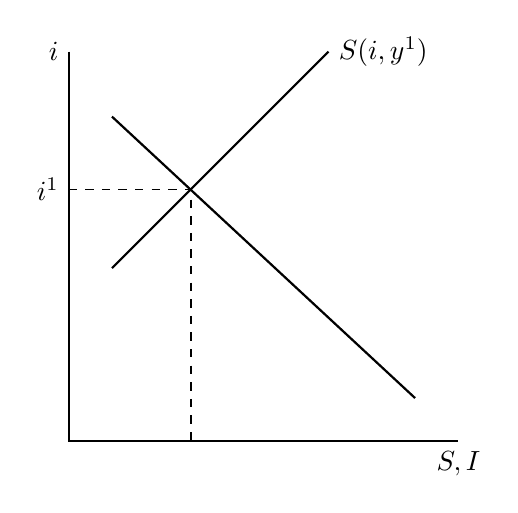
\begin{tikzpicture}[scale=0.55]
				\draw[thick] (0,9) node[left]{\( i \)} -- (0,0) -- (9,0) node[below]{\( S, I \)};
				\draw [thick] (1,7.5) -- (8,1);
				\draw [thick] (1,4) -- (6,9) node[right]{\( S(i,y^1) \)};
				\draw [dashed] (0,5.825) node[left]{\( i^1 \)} -- (2.825,5.825) -- (2.825,0);
			\end{tikzpicture}
			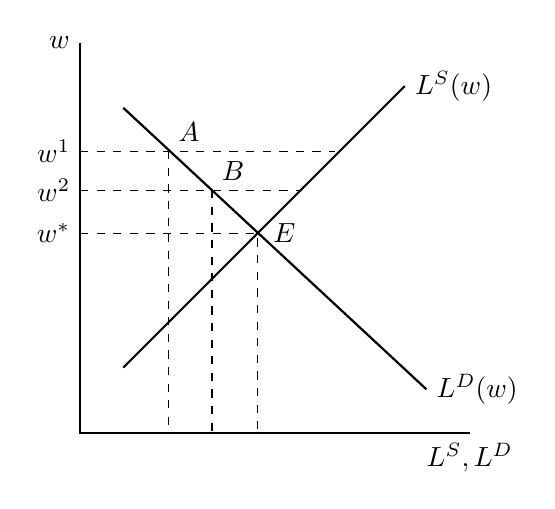
\begin{tikzpicture}[scale=0.55]
				\draw[thick] (0,9) node[left]{\( w \)} -- (0,0) -- (9,0) node[below]{\( L^S,L^D \)};
				\draw [thick] (1,7.5) -- (8,1) node[right]{\( L^D(w) \)};
				\draw [thick] (1,1.5) -- (7.5,8) node[right]{\( L^S(w) \)};
				\draw [dashed] (0,6.5) node[left]{\( w^1 \)} -- (5.9,6.5);
				\draw [dashed] (2.05,6.5) node[above right]{\( A \)} -- (2.05,0);
				\draw [dashed] (0,5.6) node[left]{\( w^2 \)}-- (5.1,5.6);
				\draw [dashed] (3.05,5.6) node[above right]{\( B \)} -- (3.05,0);
				\draw [dashed] (0,4.6) node[left]{\( w^* \)}-- (4.1,4.6) node[right]{\( \: E \)} -- (4.1,0);
			\end{tikzpicture}
		\end{figure}
\subsection{Keynes's challenge and the Development of Macroeconomics post-\textit{General Theory}}
		\begin{itemize}
			\item  Source of what Keynes regarded as critical planks in orthodox thought lie within this marginalist approach to value and distribution  
			\item Specifically, that the real wage and rate of interest ultimately reflected the balance of demand and supply of labour and capital respectively
			\item Keynes's 2 key targets in his General Theory (1936): the ``orthodox theory of employment [real wage]'' and the ``orthodox theory of the rate of interest'' 
			\item For Keynes, the real wage is determined outside the labour market
			\item Employment governed by \textit{effective demand }
			\begin{itemize}
				\item ``the principle of effective demand: \dots\: aggregate demand may be insufficient to absord the output produced from the normal use of productive capacity'' Garegnani (1988, p.69)
			\end{itemize}
			\item \( S \) governed by \( I \), through variation in the level of output and employment
			\item No automatic mechanism which would adjust \( I \) in line with the full-employment level of \( S \)
			\item Keynes viewed this as applicable not merely for the short-run
			\begin{itemize}
				\item ``We oscillate, avoiding the gravest extremes of fluctuation in employment and in prices … round an intermediate position appreciably below full-employment'' (General Theory, p.254)
			\end{itemize}
			\item \textbf{AND} for a world of price and wage flexibility 
			\item \textbf{BUT}: was Keynes's theoretical argument strong enough to support this claim?
			\item Keynes's rejection of a tendency to full-employment turned heavily on his critique of the orthodox theory of the rate of interest
			\item Problem: this critique was arguably deficient
			\item In effect, Keynes's argument comes to rest on adverse expectational effects and interest rate stickiness
			\item Both harder to defend for long-run analysis
			\item Orthodox view: Keynes's could only explain persistent unemployment by implicitly assuming rigidity in some prices/wages
			\item At the heart of the direction of macro thought and it's attitudes to policy since 
			\item Hence
			\begin{itemize}
				\item Keynesian unemployment associated with the short-run and price/wage rigidities 
				\item Principle of effective demand seen as relevant only for the short-run
			\end{itemize}
		\item By 1940's Keynes's doubts about the efficacy of wage and price flexibility in correcting unemployment seen as qualifications to orthodox theory and difficult to sustain beyond the short-run
		\item \textbf{\textit{Neoclassical synthesis}} (approx. early 1950's to early 1970's) -  Keynes's subsumed as a special ``short-run'' case within orthodox thinking
		\item Blanchard (2008) notes that it was a
		\begin{quote}
			``consensus about two beliefs … that decisions of firms and of individuals were largely rational … [but] this … did not extend to a belief in the efficient functioning of markets. The second belief was indeed that prices and wages did not adjust very quickly to clear markets''
		\end{quote}
		\item For \underline{policy}: if rigidities in wages/prices/interest rates persist \( \Rightarrow \) a role for counter-cyclical demand management
		\item ``Keynesianism'' viewed in terms of low interest elasticity of investment; high interest elasticity of money demand
		\item The synthesis reflected an underlying faith in market adjustment for the “long-run'' or trend
		\item Demand-management policy could assist in managing fluctuations in demand around this trend - its relevance belonged to the “short-run''
		\item Milgate and Eatwell (1983) refer to the Keynesianism of the post-war period as ``imperfectionist''
		\item Persistent involuntary unemployment reflecting imperfections in labour and/or product and/or financial markets
		\item Absent these imperfections or their weakening with time \( \Rightarrow \) pre-Keynesian orthodox convergence to full-employment should dominate
		\item The imperfectionist view and pre-Keynesian view share the same position on this long-run tendency
	\end{itemize}
\subsubsection{Challenges to the synthesis}
	\begin{itemize}
		\item Stagflation from the mid-1970's
		Suggested a worsening trade-off between inflation and unemployment
		\item A “shifting'' upwards of the Phillips curve
		\item \( \Rightarrow \) \textit{inter alia}, questions about the theoretical foundations of the synthesis
		\item A tension between the two “beliefs'' behind the synthesis (Blanchard, p.898) 
		\item i.e. rational maximizing agents and non-market clearing
		\item Worsening trade-off between inflation and unemployment \( \Rightarrow \) radical reinterpretation of the Phillips curve relation
		\item  Friedman-Phelps expectations-augmented Phillips curve (EAPC)
		\item Seemingly provided an account of the short-run trade-off but also how that trade-off dissipated in the long-run:
		\begin{quote}
			``the uncertainty engendered by … inflationary experience was sufficient to explain a trade-off … in the form of a short-run Phillips curve'' (Milgate and Eatwell, p. 272)
		\end{quote}
		\item This analytical approach reinforced the long-run neutrality of money (Friedman, AER, 1968): 
		\begin{quote}
			``monetary policy … cannot peg the rate of unemployment for more than very limited periods'' (p. 5)
		\end{quote}
		\begin{quote}
			``there is always a temporary trade-off between inflation and unemployment; there is no permanent trade-off … the temporary trade-off comes not from inflation per se, but from unanticipated  inflation'' (p. 11)
		\end{quote}
		\begin{quote}
			``Monetary policy can prevent money itself from being a major disturbance'' (p. 12)
		\end{quote}
		\begin{quote}
			``monetary policy can provide a stable background for the economy … [where agents] can proceed with full confidence that the average level of prices will behave in a known way in the future'' (p.13)
		\end{quote}
		\item Would lead to two different paths 
		\item Conduit for the fork in the road was ``rational expectations'' (RE) and its use particularly by Lucas à \textit{la} the Lucas supply function
		\item At one level ''an attempt to remove `uncertainty and expectations' from the catalogue of imperfections upon which'' explanations of unemployment had been based (Milgate and Eatwell, p. 273)
		\item Suggested only unanticipated macropolicy changes could have real effects
		\item With \textit{RE} applied to expected average price => anticipated monetary policy does not affect output - does not generate unanticipated inflation
		\item Agents cannot be surprised (in terms of inflation) by ``systematic monetary policy'' (Mankiw, 1990, p. 1649)
		\item  \( \Rightarrow \) ``policy ineffectiveness''
		\item Two lines of development in response to the Lucas critique: 
		\begin{itemize}
			\item those following through the logic of this critique -- \textbf{new classical macroeconomics}
			\item those not wholly prepared to do so -- \textbf{new Keynesian macroeconomics}
		\end{itemize}
		\item \textbf{New classical macroeconomics (NCM):} a rational expectations - equilibrium approach, viz., to model `as if' markets were competitive and cleared instantaneously
		\item NCM argument that disequilibrium ``implies a failure to exploit mutually beneficial trades''
		\item Economic phenomena such as fluctuations seen as explicable in terms of shocks to fundamental structural parameters e.g preferences, technology
		\item \textbf{New Keynesian macroeconomics (NKM):} the alternative -- developed through the 1980's -based on a rejection of instantaneous market clearing and questionable empirical results on  implications of the Lucas approach
		\item Impediments to market clearing the key to understanding:
		\begin{itemize}
			\item persistent divergence from full-employment 
			\item the ability of demand shocks to impact output 
			\item real effects of fiscal and monetary policy
		\end{itemize}
		\item Impediments / distortions / rigidities ``explained'' in terms of optimizing behaviour
		\item e.g. consistency of optimizing behaviour and observable price and wage sluggishness
		\item In a sense the difference between \textit{NCM} versus \textit{NKM} on the one hand and the old Keynesian versus neoclassical post-\textit{General Theory} on the other might be seen to be the degree of sophistication of the microfoundations 
		\item i.e. microfoundations about markets absent imperfections and microfoundations which explain those imperfections
		\item The question arises whether those underlying theoretical foundations - about how markets would behave without imperfections - sound?
		\item The choice between \textit{NCM} and \textit{NKM} leaves aside the position which arguably corresponds to that of Keynes:
		\begin{quote}
			demand could constrain output below its full-employment position as a part of the normal functioning of a capitalist economy in the long-run no less than the short-run and independently of rigidities in product, factor or financial markets
		\end{quote}
		\item Would entail a fundamentally different view of how markets work even at their most flexible
		\item This \textit{heterodox} position has persisted since Keynes and particularly in growth theory
	\end{itemize}

\section{Heterodox Foundations: Some Building Blocks}
\subsection{Production of Commodities by means of Commodities}
	\begin{itemize}
		\item We suppose that in a capitalist economy, capitalists are interested in maximising profit
		\item \( \Rightarrow \) comparison of \underline{profit rates} across sectors
		\item Consider the two-commodity iron/corn model
		\item With Constant Returns to Scale (CRTS), profit rates for total output of a commodity are the same as the profit rate for each unit of the commodity
		\item \( \Rightarrow \) the profit rate for each sector can be written as
		\begin{align}
			r_i &= \frac{p_i - w_m l_i - ( a_{ci} p_c +a_{ii} p_i)}{( a_{ci} p_c +a_{ii} p_i)} \notag \\ 
			r_c &= \frac{p_c - w_m l_c - ( a_{ic} p_i +a_{cc} p_c)}{( a_{ic} p_i +a_{cc} p_c)} \label{E:2.1}
		\end{align} 
		\item Absent restrictions on mobility of resources between sectors expect capitalists to exploit differentials in profit rates
		\item \( \Rightarrow \) tendency to uniformity of profit rates
		\item ``\textcolor{myred}{Long-period equilibrium}'' characterised by a uniform rate of profit across production processes
		\item \( \Rightarrow \) in Classical Political Economy and in marginalist theory up to 1930's a ``center of gravity'' in a competitive capitalist economy
		\item  Rearranging \cref{E:2.1} and with \( r_i = r_c = r \) gives:
		\begin{align}
			p_i &= (a_{ci} p_c + a_{ii} p_i) (1 + r) + w_m l_i \notag \\
			p_c &= (a_{ic} p_i + a_{cc} p_c) (1 + r) + w_m l_c \label{E:2.2}
		\end{align}
		\item Note: if technical conditions of  production are given \( \Rightarrow \) 2 equations with 4 unknowns
		\item Can reduce \cref{E:2.2} to relative values by setting a numeraire, e.g. corn, \( p_c = 1 \)
		\begin{align}
			(a_{ci} p_c + a_{ii} p_i) (1 + r) + w_m l_i &= p_{ic} \notag \\
			(a_{ic} p_i + a_{cc} p_c) (1 + r) + w_m l_c &= 1 \label{E:2.3}
		\end{align}
		where \( w = \frac{w_m}{p_c} \) and \( p_{ic} = \frac{p_i}{p_c} \)
		\item \( \Rightarrow \) 2 equations with 3 unknowns
		\item Alternatively, could set \( w_m \) as numeraire \( \Rightarrow \) 
		\begin{align}
			(a_{ci} p_{cw} + a_{ii} p_{iw}) (1 + r) + l_i &= p_{iw} \notag \\
			(a_{ic} p_{iw} + a_{cc} p_{cw}) (1 + r) + l_c &= p_{cw} \label{E:2.4}
		\end{align}
		where \( p_{iw} = \frac{p_i}{w_m} \) and \( p_{cw} = \frac{p_c}{w_m} \)
		\item For both \cref{E:2.3} and \cref{E:2.4}, setting one unknown exogenously, allows the remaining two unknowns to be determined by the price equations
		\item So which variable - real wage, rate of profit or relative price - should be exogenous? 
	\end{itemize}
\subsubsection{The \textit{n}-commodity case}
	\begin{itemize}
		\item The technique of production is given by
		\[
			\begin{bmatrix}
				a_{11} & a_{12} & a_{13} & \cdots & a_{1n} \\
				a_{21} & a_{22} & a_{23} & \cdots & a_{2n} \\
				a_{31} & a_{32} & a_{33} & \cdots & a_{3n} \\
				\vdots & \vdots & \vdots & \ddots & \vdots \\
				a_{n1} & a_{n2} & a_{n3} & \cdots & a_{nn} \\
				I_1 & I_2 & I_3 & \dots & I_4
			\end{bmatrix}
		\]
		\item \( \Rightarrow \) the n-sector price system is
		\begin{gather}
			\left( a_{11} p_1 + a_{21} p_2 + a_{31} p_3 + \dots + a_{n1} p_n \right) \left( 1 + r \right) + w_m l_1 = p_1 \notag \\ 
			\left( a_{12} p_1 + a_{22} p_2 + a_{32} p_3 + \dots + a_{n2} p_n \right) \left( 1 + r \right) + w_m l_2 = p_2 \notag \\ 
			\left( a_{13} p_1 + a_{23} p_2 + a_{33} p_3 + \dots + a_{n3} p_n \right) \left( 1 + r \right) + w_m l_3 = p_3 \notag \\
			\vdots \qquad \vdots \qquad \vdots \qquad \vdots \qquad \vdots \qquad \vdots \qquad \vdots \qquad \vdots \notag \\
			\left( a_{1n} p_1 + a_{2n} p_2 + a_{3n} p_3 + \dots + a_{nn} p_n \right) \left( 1 + r \right) + w_m l_n = p_n \label{E:2.5}
		\end{gather}
		\item With commodity \( k \) as numeraire \( (p_k = 1) \Rightarrow n-1 \) relative prices (i.e. price of commodities other than \( k \) in terms of commodity k), real wage (in terms of \( k \)) and rate of profit
		\item \( \Rightarrow n+1 \) unknowns in \( n \) equations
		\item Note similarity with two-sector case
		\item This approach to relative prices and distribution referred to as ``\textcolor{myred}{surplus}'' or ``\textcolor{myred}{modern classical}''
		\begin{enumerate}[(i)]
			\item relative prices and remaining distributive variable are fully determined by the price system: i.e. by technical conditions and the value of the exogenous distributive variable 
			\item resulting relative prices are ``normal'' or ``long-period equilibrium'' prices
			\item relative prices can only change if technical conditions or the value of the exogenous distributive variable change
			\item changes in demand for a commodity affect it's long-period relative price only where they affect technical conditions or the exogenous distributive variable
			\item income distribution is partly exogenous to the price system  (in contrast with orthodox approaches)
		\end{enumerate}
		\item In the words of Garegnani, (in describing how Sraffa himself arrived at this theoretical position)
		\begin{quote}
			“the basic result [is] …. that essentially, the physical conditions of production of the commodities [plus a given real wage or rate of profit] and the need to allow production to be repeated [and thus for relative prices to be such as to allow for production to be repeated] are sufficient to determine relative prices quite independently of what are generally understood as `demand and supply forces'''  (“On a turning point in Sraffa's theoretical and interpretative position of the 1920's'', \textbf{Euro. Journal of the History of Economic Thought}, Sept. 2005, p. 469)
		\end{quote}
	\end{itemize}
\subsubsection{Closing the Price System in the Iron/Corn Case}
	\begin{itemize}
		\item  Let
		\begin{equation}
			w_m = X \cdot p_c \qquad \therefore w = X \label{E:2.6}
		\end{equation}
		\item With \( X \) given, and taking corn as the numeraire,
		\begin{align}
			(a_{ci} + a_{ii} p_{ic}) (1 + r) + X \: l_i &= p_{ic} \notag \\
			(a_{ic} p_{ic} + a_{cc}) (1 + r) + X \: l_c &= 1 \label{E:2.7}
		\end{align}
		\item Alternatively, with \( w_m = X_c p_c + X_i p_i \text{ and } X_c \text{ and } X_i\) given, and corn as numeraire,
		\begin{align}
			(a_{ci} + a_{ii} p_{ic}) (1 + r) + l_i ( X_c + p_{ic} X_i) &= p_{ic} \notag \\
			(a_{ic} p_{ic} + a_{cc}) (1 + r) + l_c ( X_c + p_{ic} X_i) &= 1 \label{E:2.8}
		\end{align}
		\item with \( r \) exogenously given in \cref{E:2.7}, the relative price and X (the real wage in terms of corn) are determined endogenously
		\item Interesting question - what forces govern the exogenous distributive variable?
	\end{itemize}
\subsubsection{The real wage - rate of profit relation}
	\begin{itemize}
		\item Consider the two-sector case:
		\begin{gather}
			(a_{11} p_1 + a_{21} p_2) (1 + r) + w_m l_1 = p_1 \notag \\
			(a_{21} p_1 + a_{22} p_2) (1 + r) + w_m l_2 = p_2 \label{E:2.9}
		\end{gather}
		\item  Assume \( p_2 = 1 \), so that
		\begin{align}
			(a_{11} p_{12} + a_{21}) (1 + r) + w_m l_1 &= p_{12} \notag \\
			(a_{21} p_{12} + a_{22}) (1 + r) + w_m l_2 &= 1 \label{E:2.10}
		\end{align}
		where \( w_2 = \frac{w_m}{p_2} \) and \( p_{12} = \frac{p_1}{p_2} \)
		\item Rearranging equations (\ref{E:2.10}),
		\begin{equation}
			w_2 = \frac{(a_{11} a_{22} - a_{12} a_{21}) (1 + r)^2 - (a_{11} + a_{22}) (1 + r) + 1}{(l_1 a_{12} - l_2 a_{11}) (1 + r) + l_2} \label{E:2.11}
		\end{equation}
		\item Or, alternatively, with \( p_1 = 1 \)
		\begin{align}
			(a_{11} + a_{21} p_{21}) (1 + r) + w_m l_1 &= 1 \notag \\
			(a_{12} + a_{21} p_{21}) (1 + r) + w_m l_2 &= p_{21} \label{E:2.12}
		\end{align}
		where \( w_1 = \frac{w_m}{p_1} \) and \( p_{21} = \frac{p_2}{p_1} \)
		\begin{equation}
			w_1 = \frac{(a_{11} a_{22} - a_{12} a_{21}) (1 + r)^2 - (a_{11} + a_{22}) (1 + r) + 1}{(l_2 a_{21} - l_1 a_{22}) (1 + r) + l_1} \label{E:2.13}
		\end{equation}
		\item With
		\[
			\frac{dw_1}{d_r} < 0 \text{ and } \frac{dw_2}{d_r} < 0
		\]
		\item  For example, consider equations (\ref{E:2.12}) with the second equation (commodity 2) rewritten as
		\[
			\frac{1}{p_{21}} (a_{12} (1 + r) + w_1 l_2) = 1 - a_{22} (1 + r)
		\]
		so that, if both \( w_1 \) and \( r \) rise, \( p_{21} \) must rise. But from the first equation (\ref{E:2.12})
		\item If both \( w_1 \) and \( r \) rise, \( p_{21} \) must fall. Hence \( w \) and \( r \) cannot both rise
		\item Note: the \textit{w-r} relation is inverse regardless of the numeraire
	\end{itemize}
\subsubsection{The Maximum Rate of Profit, Maximum Real Wage and Relative Prices}
	\begin{itemize}
		\item With an inverse \textit{w-r}, the maximum rate of profit will be associated with \( w = 0 \). Substituting this condition in \cref{E:2.11} and \cref{E:2.13} yields
		\begin{equation}
			(a_{11}a_{22} - a_{12} a_{21}) (1 + r)^2 - (a_{11} + a_{22})(1 + r) + 1 = 0 \label{E:2.14}
		\end{equation}
		\item Note that the max. \( r (= R) \) is independent of the numeraire and labour input requirements
		\item Maximum real wage will be associated with \( r = 0 \). Substituting in \cref{E:2.11} and \cref{E:2.13} yields respectively
		\begin{gather}
			w_2 = \frac{( 1 - a_{11}) (1 -a_{22}) - a_{12} a_{21}}{(l_1 a_{12} - l_2 a_{11}) + l_2} \notag \\
			w_1 = \frac{( 1 - a_{11}) (1 -a_{22}) - a_{12} a_{21}}{(l_2 a_{21} - l_2 a_{22}) + l_1} \label{E:2.15}
		\end{gather}
		\item \( \Rightarrow \) maximum real wage depends on the numeraire
		\item Summing so far: for each technique (i.e. set of \( a_{ij} \)'s and \( l_i \)'s) one can construct a price system which yields:
		\begin{enumerate}[(i)]
			\item an inverse relation between w and r, whatever the numeraire; 
			\item a maximum rate of profit independent of the numeraire; and 
			\item a maximum real wage dependent on the numeraire 
		\end{enumerate}
		\begin{figure}[H]
			\centering
			\begin{tikzpicture}[scale=0.55]
			\draw [thick] (0,9) node[left]{\(w\)} -- (0,0) -- (9,0) node[below]{\(r\)};
			\draw [thick] (0,6) node[left]{\(W_2\)} .. controls (4,5.75) and (7.25,2.5) .. (7.5,0) node[below]{\(R\)};
			\draw [thick, dotted] (0,4) node[left]{\( W_1 \)}.. controls (4,3.75) and (7.25,2) .. (7.5,0);
		\end{tikzpicture}
		\end{figure}
		\item From \cref{E:2.11} and \cref{E:2.13} respectively
		\begin{gather*}
			\frac{p_1}{w_m} = \frac{(l_2 a_{21} - l_1 a_{22}) (1+r) + l_1}{(a_{11} a_{22} - a_{12} a_{21}) (1+r)^2 - (a_{11} + a_{22}) (1 + r) + 1} \\
			\frac{p_2}{w_m} = \frac{(l_1 a_{12} - l_2 a_{11}) (1+r) + l_2}{(a_{11} a_{22} - a_{12} a_{21}) (1+r)^2 - (a_{11} + a_{22}) (1 + r) + 1} 
		\end{gather*}
		so that
		\begin{equation}
			\frac{w_2}{w_1} = \frac{p_1}{p_2} = p_{12} = \frac{(l_2 a_{21} - l_1 a_{22}) (1 + r) + l_1}{(l_1 a_{12} - l_2 a_{11}) (1 + r) + l_2} \label{E:2.16}
		\end{equation}
		where
		\begin{equation}
			\frac{dp_{12}}{dr} \lesseqgtr 0 \label{E:2.17}
		\end{equation}
		depending on the technical conditions of production 
		\item \textit{Note: any set of relative prices will in general  presuppose a particular income distribution}
		\item  Note also that where
		\begin{align*}
			l_2 a_{21} &= l_1 a_{22}\\
			\frac{l_2}{a_{22}} & = \frac{l_1}{a_{21}}\\
			l_1 a_{12} &= l_2 a_{11}\\
			\frac{l_1}{a_{11}} & = \frac{l_2}{a_{12}}
		\end{align*}
		so that \( \frac{dp_{12}}{dr} = 0 \)
		\item More generally, consider the \( n \)-commodity case \cref{E:2.5} with \( w_m = 1 \), and consider \( p_j^1 \)
		\item From Pasinetti (1977, pp. 82-83), \( \frac{dp_{12}}{dr} \gtrless 0 \)  according to whether 
		\[
			\left[ p_1 \sum_{i = 1}^{n} a_{ij} p_i - p_j \sum_{i = 1}^{n} a_{i1} p_i \right] + (1+r) \left[ p_1 \sum_{i = 1}^{n} a_{ij} \frac{dp_i}{dr} - p_j \sum_{i = 1}^{n} a_{i1} \frac{dp_i}{dr} \right] \gtrless 0
		\]
		\item Note: 1st term relates to technology solely of the two sectors - \( j \) and 1
		\item But 2nd term brings into play technologies in other sectors, via effects of \( \Delta \)'s in \( r \) on other prices
		\item Where \( r = 0 \) and thus where \( w = W \)
		\begin{equation}
			p_{12} = \frac{l_2 a_{21} - l_1 a_{22} + l_1}{l_1 a_{12} - l_2 a_{11} + l_2} \label{E:2.18}
		\end{equation}
		\item  In this case relative prices depend on the relative quantities of embodied labour (direct and indirect)
	\end{itemize}
\subsubsection{Basics and Non-basics}
	\begin{itemize}
		\item Are some commodities ``more important'' than others in determining income distribution? 
		\item Sraffa's (1960) distinction between basic and non-basic commodities addresses this question
		\item Basic commodities are required directly or indirectly in the production of \underline{all} commodities
		\item  Consider a 3-commodity economy with the following technical conditions:
		\[
		A =
		\begin{bmatrix}
			a_{11} & a_{12} & a_{23} \\
			a_{21} & a_{22} & a_{23} \\
			0 & 0 & 0 \\
			I_1 & I_2 & I_3
		\end{bmatrix}
		\]
		\item \( \Rightarrow \) commodities 1 and 2 are basic; commodity 3 is non-basic
		\item  The price system is:
		\begin{gather}
			(a_{11} p_1 + a_{21} p_2 + 0p_3) (1+r) + w_m l_1 = p_1 \notag \\
			(a_{12} p_1 + a_{22} p_2 + 0p_3) (1+r) + w_m l_2 = p_2 \notag \\
			(a_{13} p_1 + a_{23} p_2 + 0p_3) (1+r) + w_m l_3 = p_3 \label{E:2.19}
		\end{gather}
		\item  Taking commodity 1 as numeraire: 
		\begin{align}
			(a_{11} + a_{21} p_{21} + 0p_{31}) (1+r) + w_1 l_1 &= 1 \notag \\
			(a_{12} + a_{22} p_{21} + 0p_{31}) (1+r) + w_1 l_2 &= p_{21} \notag \\
			(a_{13} + a_{23} p_{21} + 0p_{31}) (1+r) + w_1 l_3 &= p_{31} \label{E:2.20}
		\end{align}
		\item Consider first two price equations \( \Rightarrow \) 2 equations in \( p_{21}, r \) and \( w_1 \)
		\item \( \Rightarrow \) with \( w_1 \) exogenous for example, \( p_{21} \) and \( r \) are fully determined
		\item Substituting solved value for \( r \) and \( p_{21} \) in 3rd equation determines \( p_{31} \)
		\item \( \Rightarrow \) \textbf{relative price of basic commodities and endogenous distributive variable can be determined by reference exclusively to the conditions of production of basic commodities}
		\item Note, taking either the 2\textsuperscript{nd} and 3\textsuperscript{rd} equations or the 1\textsuperscript{st} and 3\textsuperscript{rd} equations, we would have two equations in 4 unknowns and could not therefore solve as before by taking  one of the distributive variables as exogenous
		\item \textbf{Conditions of production of non-basics are relevant only to their own prices and those of other non-basics into which they enter as input}
		\item Consider a change in technical conditions of a commodity (e.g. due to an invention)
		\item If the commodity is basic -- all prices in the system are affected
		\item If the commodity is non-basic -- only its own price and that of other non-basics into which it is an input are affected
		\item Problems with partial equilibrium micro analysis: e.g. a tax on the production of a basic affects all prices
		\item \( \Rightarrow \) violates \textit{ceteris paribus} behind supply curve
	\end{itemize}
\subsubsection{Some Comparisons with Conventional Theory}
	\begin{itemize}
		\item In particular, with orthodox demand and supply explanation of relative prices?
		\item Analysis so far \( \Rightarrow \) changes in the composition of demand do not affect relative prices unless they affect the exogenous distributive variable, \( a_{ij} \)'s or \( l_i \)'s
		\item Orthodox theory however allows for such an effect:
		\item e.g. a rise in demand for a particular commodity, relative to other commodities, increases relative demand for factors used more intensively in the production of this commodity
		\item  \( \Rightarrow \) relative price of those factors rises
		\item \( \Rightarrow \) unit cost of production rises
		\item Hence, even with CRTS (i.e. constant \( a_{ij} \)'s and \( l_i \)'s) \( \Rightarrow \) “supply price'' rises with output
		\( \Rightarrow \) \textbf{dependence of price on demand in an orthodox framework, at least with CRTS, is a reflection of the dependence of the return to factors of production and hence income distribution on demand and supply}
		\item There a role for demand and supply interaction in a modern classical approach -- in disequilibrium, rather than equilibrium!
		\item  In an orthodox framework demand and supply (interpreted as functional relations) interaction governs the equilibrium price as well and the out-of-equilibrium price 
		\item In a modern classical approach demand and supply interaction affects out-of-equilibrium prices
		\item \textbf{BUT} equilibrium prices are determined by technical conditions and an exogenous distributive variable
	\end{itemize}
\subsection{The Choice of Technique: A Preliminary Analysis}
	\begin{itemize}
		\item Consider the two-commodity case, with 3 available techniques differing in the method used to produce commodity 2
		\item Each technique \( \Rightarrow \) \textit{w-r} curve for a particular numeraire
		\item  Assume the same numeraire for each technique
		\item \( \Rightarrow \) can compare \textit{w-r} relations
		\item  Suppose the techniques are:
		\[
		A^\alpha =
		\begin{bmatrix}
			a_{11} & a_{12}^\alpha \\
			a_{21} & a_{22}^\alpha
		\end{bmatrix}
		\quad
		A^\beta =
		\begin{bmatrix}
			a_{11} & a_{12}^\beta \\
			a_{21} & a_{22}^\beta
		\end{bmatrix}
		\quad
		A^\delta =
		\begin{bmatrix}
			a_{11} & a_{12}^\delta \\
			a_{21} & a_{22}^\delta
		\end{bmatrix}
		\]
		\item  Which technique is chosen at different \( w-r \) combinations? If \( w \) as exogenous, presumably technique yielding highest rate of profit
		\item What if \( r \) is exogenous? 
		\item Consider for example \( r = \bar{r_0} \)
		\begin{align*}
			w^\delta > w^\beta &\Rightarrow \frac{w_m}{p^\delta} > \frac{w_m}{p^\delta} \\
			&\Rightarrow p^\delta < p^\beta
		\end{align*}
	\end{itemize}
	\begin{figure}[H]
		\centering
		\begin{tikzpicture}[scale=0.55]
			\draw [thick] (0,9) node[left]{\(w\)} -- (0,0) -- (9,0) node[below]{\(r\)};
			\draw [thick] (0,6) .. controls (0.5,2) and (4.5,0.5) .. (9,0.5);
			\draw[<-] (8,0.7) -- (8.3,1.3) node[right]{\( \delta \)};
			\draw [thick,dashed] (0,8.5) .. controls (0.5,2.5) and (3.5,0.5) .. (7,0);
			\draw[<-] (2,3) -- (2.5,3.5) node[right]{\( \beta \)};
			\draw [thick,dash dot] (0.5,8.5) .. controls (1,2) and (2.5,0.5) .. (5,0);
			\draw[<-] (0.7,8) -- (1.3,8.3) node[right]{\( \alpha \)};
			\draw [thick, dotted, color=mygreen] (0,1.3) node [left,color=black] {\(\bar{w}\)}-- (4,1.3) -- (4,0) node [below,color=black]{\( \bar{r_0} \)};
			\draw[thick, dotted, color=mygold] (2.6,0) node [below,color=black]{\( \bar{r_1} \)} -- (2.6,2);
		\end{tikzpicture}
	\end{figure}
	\begin{itemize}
		\item Note: adjacent techniques at a switch point will in general differ in the method of producing \underline{only one} of the commodities
		\item \( \Rightarrow \) in the 2-commodity case, at the switch point there are three unknowns between the two price systems -- \( p_{21}, w_1 \) and \( r \)
		\item At \( r = \bar{r_1} \)
		\begin{align*}
			( a_{11}^\beta +  a_{21}^\beta p_{21} ) (1 + r) + w_1 l_1 &= 1 \\
			( a_{12}^\beta +  a_{22}^\beta p_{21} ) (1 + r) + w_1 l_2 &= p_{21} \\
			( a_{11}^\delta +  a_{21}^\delta p_{21} ) (1 + r) + w_1 l_1 &= 1 \\
			( a_{12}^\delta +  a_{22}^\delta p_{21} ) (1 + r) + w_1 l_2 &= p_{21}
		\end{align*}
		\item \( \Rightarrow \) require three equations from the two systems \( \Rightarrow \) only one equation can be different between the two systems
		\item Applying this choice of technique analysis to basic commodities, a lower price for one commodity under one method \( \Rightarrow \) a lower price for all commodities using that method
		\item \(\Rightarrow  \) ranking of techniques according to profitability as \textit{w} falls and \textit{r} rises is the same regardless of the numeraire
		\item Moreover, the ranking of techniques is independent of the technique in which prices are expressed 
		\item e.g. at \( r^* \) the relative cheapness of techniques \( \delta \) and \( \beta \) should be the same whether costs of production are compared using \( p^\delta \) or \( p^\beta \)
		\item \( \Rightarrow \) at \( r^* \) using either the real wage \( w^\beta \) or \( w^\delta \) to calculate prices for each technique would show that technique \( \delta \) yields lower prices than technique \( \beta \)
	\end{itemize}
	\begin{figure}[H]
		\centering
		\begin{tikzpicture}[scale=0.55]
			\draw [thick] (0,9) node[left]{\(w\)} -- (0,0) -- (9,0) node[below]{\(r\)};
			\draw [thick] (0,6) .. controls (0.5,2) and (4.5,0.5) .. (9,0.5);
			\draw[<-] (8,0.7) -- (8.3,1.3) node[right]{\( \delta \)};
			\draw [thick,dashed] (0,8.5) .. controls (0.5,2.5) and (3.5,0.5) .. (7,0);
			\draw[<-] (2,3) -- (2.5,3.5) node[right]{\( \beta \)};
			\draw [thick, dotted] (0,1.3) node [above right]{\(w^\delta\)} -- (4,1.3);
			\draw [thick, dotted] (0,0.95) node [below right]{\(w^\beta\)} -- (4,0.95);
			\draw [thick, dotted, color=mygreen] (4,1.3) -- (4,0) node [below, color=black]{\( r^* \)};
		\end{tikzpicture}
	\end{figure}
	\begin{itemize}
		\item \( \Rightarrow \) at \( r^* \) using either the real wage \( w^\beta \) or \( w^\delta \) to calculate prices for each technique would show that technique \( \delta \) yields lower prices than technique \( \beta \)
		(see for example, Garegnani, 1970, p. 411n)
		\item Suggests the technique which would dominate in a long-period equilibrium, for a given rate of profit, generates the highest real wage
		\item \( \Rightarrow \) \textit{dominant technique will be the technique generating the highest rate of profit at the given real wage or the highest real wage at the given rate of profit}
		\item Suggests that the relevant portion of the set of \textit{w-r} curves (representing available techniques) is the outermost envelope of this set
	\end{itemize}
	\begin{figure}[H]
		\centering
		\begin{tikzpicture}[scale=0.55]
			\draw [thick] (0,9) node[left]{\(w\)} -- (0,0) -- (9,0) node[below]{\(r\)};
			\draw [thick] (0,6) .. controls (0.5,2) and (4.5,0.5) .. (9,0.5);
			\draw[<-] (8,0.7) -- (8.3,1.3) node[right]{\( \delta \)};
			\draw [thick,dashed] (0,8.5) .. controls (0.5,2.5) and (3.5,0.5) .. (7,0);
			\draw[<-] (2,3) -- (2.5,3.5) node[right]{\( \beta \)};
			\draw [thick,dash dot] (0.5,8.5) .. controls (1,2) and (2.5,0.5) .. (5,0);
			\draw[<-] (0.7,8) -- (1.3,8.3) node[right]{\( \alpha \)};
			\draw [smooth,very thick,color=mygreen] plot coordinates {(0.5,8.5)(0.8,5.8)(1.3,3.75)(1.85,2.8)(2.6,2)(4,1.3)(6,0.75)(7.75,0.55)(9,0.5)};
			\draw (0,1.3) node [left] {\(\bar{w}\)}-- (4,1.3) -- (4,0) node [below]{\( \bar{r_0} \)};
		\end{tikzpicture}
	\end{figure}

\section{Capital-Theoretic Issues and Conventional Macroeconomic Theory}
\subsection{Distribution, Input Proportions and the Choice of Technique}
	\begin{itemize}
		\item Consider a simplified two-sector model, with only labour and commodity two used as inputs:
		\begin{align}
			a_{21}p_2 (1 + r) + w_m l_1 &= p_1 \notag \\
			a_{22}p_2 (1 + r) + w_m l_2 &= p_2 \label{E:3.1}
		\end{align}
		\item Taking commodity 1 as numeraire  
		\begin{align}
			a_{21}p_2 (1 + r) + w l_1 &= 1 \notag \\
			a_{22}p_2 (1 + r) + w l_2 &= p_{21} \label{E:3.2}
		\end{align}
		\item where
		\begin{equation}
			w = \frac{1 - a_{22} (1 + r)}{l_1 + (l_2 a_{21} - l_1 a_{22}) (1 + r)} \quad \frac{dw}{dr} < 0 \label{E:3.3}
		\end{equation}
		and
		\begin{equation}
			p_{21} = \frac{(1_2 a_{21} - l_1 a_{22}) w + a_{22}}{a_{21}} \label{E:3.4}
		\end{equation}
		so that
		\begin{equation}
			\frac{dp_{21}}{dw} = l_2 a_{21} - l_1 a_{22} \label{E:3.5}
		\end{equation}
		\item It follows from \cref{E:3.5} that
		\begin{equation}
			\frac{dp_{21}}{dw} \gtreqless \quad \text{where} \quad l_2 a_{21} - l_1 a_{22} \gtreqless 0 \label{E:3.6}
		\end{equation}
		\item and therefore
		\begin{equation}
			\frac{dp_{21}}{dw} \gtreqless \quad \text{where} \quad \left( \frac{a_{21}}{l_1} \right) \gtreqless \left( \frac{a_{22}}{l_2} \right) \label{E:3.7}
		\end{equation}
		\item Assume all wages are spent and that all profits are spent on consumption \( \Rightarrow \) a stationary economy 
		\item The wage rate is the wage bill per worker 
		\item \( \Rightarrow \) at \( r = 0, w = \) net product per worker
		\item \( \Rightarrow w_{max} = Y/L \)
		\item At \( r_1, w_1 \) profit per worker = \( w_{max} w_1 \)
		\item Slope of \( w_{max}X = \frac{(w_{max}w_1)}{(w_1 X)} = \frac{\text{profit per worker  at } X}{\text{rate of profit at } X} = \text{ value of capital per worker at } X \)
	\end{itemize}
	\begin{figure}[H]
		\centering
		\begin{tikzpicture}[scale=0.55]
			\draw [thick] (0,9) node[left]{\(w\)} -- (0,0) -- (9,0) node[below]{\(r\)};
			\draw [thick, dashed, color=myred] (0,3.5) node [left, color=black]{\( w_1 \)} -- (6.2,3.5) node [above right,color=black]{\( X \)} -- (6.2,0) node [below, color=black]{\( r_1 \)};
			\draw[thick, dashed, color=mygreen] (0,7.5) -- (6.2,3.5);
			\draw [thick] (0,7.5) node[left]{\(w_{max}\)} to [in=100,out=-10] (7.5,0) node[below]{\(R\)};
		\end{tikzpicture}
	\end{figure}
	\begin{itemize}
		\item Rising value of capital per worker as r increases
		\item \( p_{21} \) rises as r rises
	\end{itemize}
	\[
		\frac{a_{22}}{l_2} > \frac{a_{21}}{l_1}
	\]
	\begin{figure}[H]
		\centering
		\begin{tikzpicture}[scale=0.55]
			\draw[thick, dashed, color=myred] (0,7.5) -- (5.4,4.6);
			\draw[thick, dashed, color=myred] (0,7.5) -- (7,1.9);
			\draw [thick,color=myblue] (0,7.5) node[left,color=black]{\(w_{max}\)} to [in=100,out=-10] (7.5,0) node[below,,color=black]{\(R\)};
			\draw [thick] (0,9) node[left]{\(w\)} -- (0,0) -- (9,0) node[below]{\(r\)};
		\end{tikzpicture}
	\end{figure}
	\begin{itemize}
		\item Falling value of capital per worker as r increases
		\item \( p_{21} \) falls as r rises
	\end{itemize}
	\[
	\frac{a_{22}}{l_2} < \frac{a_{21}}{l_1}
	\]
	\begin{figure}[H]
		\centering
		\begin{tikzpicture}[scale=0.55]
			\draw [thick,color=myblue] (0,7.5) node[left,color=black]{\(w_{max}\)} to [in=-190,out=-80] (7.5,0) node[below,,color=black]{\(R\)};
			\draw[thick, dashed, color=myred] (0,7.5) -- (2.4,2.6);
			\draw[thick, dashed, color=myred] (0,7.5) -- (5,0.8);
			\draw [thick] (0,9) node[left]{\(w\)} -- (0,0) -- (9,0) node[below]{\(r\)};
		\end{tikzpicture}
	\end{figure}
\subsection{Heterogeneous Capital, the Production Function and the Choice of Technique}
	\begin{itemize}
		\item  Assume that there exists alternative techniques, each involving the production of two commodities - a wage-good and a capital-good - each by means of labour and the capital-good 
		\item The capital-good produced by each technique is specific to that technique \(\Rightarrow\) it is produced by a combination \textbf{\textcolor{myred}{of labour and the capital good}} specific to that technique
		\item In the ``actual'' economy, the technique of production changes continuously \(\Rightarrow\) technological frontier is smooth and continuous
		\item The ``actual'' economy can be described by a number of key relations:
		\begin{gather}
			w = e(r) \notag\\
			q = q(r) \label{E:3.8}\\
			k = k(r) \notag 
		\end{gather}
		\item Equation \ref{E:3.8} represent three features of that envelope:
		\begin{enumerate}[(i)]
			\item the inverse relation between \textit{w-r} as we move down the envelope involving switches in the technique of production, \( w = e(r) \)
			\item the relation between net product per worker (the maximum real wage for the technique in use - i.e. the vertical intercept of the \textit{w-r} curve corresponding to the technique in use at a particular rate of profit) and the rate of profit, \( q = q(r) \)
			\item the relation between the value of capital per worker (the slope of the line drawn from the maximum real wage of the \textit{w-r} curve corresponding to the technique in use and the point on the envelope) and the rate of profit, \( k = k(r) \).
		\end{enumerate}
	\end{itemize}
	\begin{figure}[H]
		\centering
		\begin{tikzpicture}[scale=0.55]
			\draw [smooth,thick,color=cyan] plot coordinates {(0,8)(1.2,7)(2,5.6)(3.3,4.3)(4.3,3.6)(5.4,2.9)(6.3,1.5)(8,0)};
			\draw [thick,color=myblue] (0,5.5) node[left,color=black]{\(q_1\)} .. controls (4.25,5.25) and (4.75,2) .. (5,0);
			\draw[thick, dashed, color=myred] (0,5.5) -- (3.3,4.3);
			\draw[dashed] (0,4.3) node[left]{\( w_1 \)} -- (3.3,4.3) -- (3.3,0) node[below]{\( r_1 \)};
			\filldraw[black] (3.3,4.3) circle (3pt) node[above right]{\( A \)};
			\draw [thick,color=myblue] (0,3.5) node[left,color=black]{\(q_2\)} .. controls (4.25,3.25) and (6.75,2) .. (7,0);
			\draw[<-] (0.5,7.7) -- (2,9) node[right]{\( E \)};
			\draw[thick, dashed, color=myred] (0,3.5) -- (6.3,1.5);
			\draw[<-] (1.8,4.9) -- (3.3,7.5) node[right]{slope = \( k_1 \)};
			\draw[dashed] (0,1.5) node[left]{\( w_2 \)} -- (6.3,1.5) -- (6.3,0) node[below]{\( r_2 \)};
			\filldraw[black] (6.3,1.5) circle (3pt) node[above right]{\( B \)};
			\draw[<-] (4,2.4) -- (5.3,4.5) node[right]{slope = \( k_2 \)};
			\draw [thick] (0,9) node[left]{\(w\)} -- (0,0) -- (9,0) node[below]{\(r\)};
		\end{tikzpicture}
	\end{figure}
	\begin{itemize}
		\item Consider the constant returns to scale production function \( Y = F(K, L) \) together with the conditions
		\begin{enumerate}[(i)]
			\item \( MPL = \delta Y/ \delta L = w \)
			\item \( MPK = \delta Y/ \delta K = r \)
		\end{enumerate}
		\item \textcolor{myred}{Under what conditions does such a ``surrogate'' function along with conditions (i) and (ii) imply relations between  \textit{w}, \textit{r}, \textit{q} and \textit{k} which correspond with those of the ``actual'' economic system?}
		\item If the function is to replicate the ``actual'' \textit{w-r} and \textit{q-r} relations, conditions (i) and (ii) imply
		\begin{gather}
			MP_L = e(MP_K) \qquad \therefore \frac{\partial Y}{\partial L} = e\left(\frac{\partial Y}{\partial L}\right) \label{E:3.9} \\
			\intertext{and}
			\frac{Y}{L} = q(MP_K) \label{E:3.10}
		\end{gather}
		\item Constant returns to scale implies
		\begin{equation}
			\frac{Y}{L} = \frac{\partial Y}{\partial L} + \left(\frac{\partial Y}{\partial K} \cdot \frac{K}{L}\right) \label{E:3.11}
		\end{equation}
		\item The slope of \( E \) for the ``actual'' system is given by \( dw/dr \Rightarrow \) if the marginal productivity conditions apply, the slope of \( E \) predicted by the surrogate production function is
		\begin{equation}
			e'(r) = \frac{dw}{dr} = \frac{d\left(\frac{\partial Y}{\partial L}\right)}{d\left(\frac{\partial Y}{\partial K}\right)} \label{E:3.12}
		\end{equation}
		\item Equation \ref{E:3.11} can be rearranged so that
		\begin{equation}
			\frac{\partial Y}{\partial L} = \frac{Y}{L} - \left(\frac{\partial Y}{\partial K} \cdot \frac{K}{L}\right) \Rightarrow \left(w = \frac{Y}{L} - r\cdot\frac{K}{L}\right) \label{E:3.13}
		\end{equation}
		\item Differentiating \cref{E:3.13} with respect to \( \delta Y/\delta K \) gives
		\begin{equation}
			\frac{d\left(\frac{\partial Y}{\partial L}\right)}{d\left(\frac{\partial Y}{\partial K}\right)} = -\frac{K}{L} \label{E:3.14}
		\end{equation}
		\item Note, \cref{E:3.12}, this differential is what the surrogate production function would identify as the slope of the technological frontier, \( E \), so that
		\begin{equation}
			\frac{K}{L} = -e'(r) \label{E:3.15}
		\end{equation}
		\item \textcolor{myred}{Hence, if \textit{w} and \textit{r} are equal to the corresponding MP's, and if the production function is to replicate the technological frontier \textit{E} of the ``actual'' system, then the value of capital per worker predicted by the production function at the rate of profit \textit{r} is the slope of \textit{E} at that rate of profit}
		\item In other words, at a particular rate of profit, the aggregate production would equate the absolute value of the slope of the envelope or technological frontier at that rate of profit with the capital to labour ratio in the economy at that rate of profit.
	\end{itemize}
	\begin{figure}[H]
		\centering
		\begin{tikzpicture}[scale=0.55]
			\draw [smooth,thick,color=cyan] plot coordinates {(0,7)(0.5,6.5)(0.9,6)(1.3,4.9)(2.6,4)(3.1,3.3)(3.6,2.3)(5.2,1.3)(6.5,0)};
			\draw [thick,dashed,color=myred] (0,7.25) -- (5.25,0);
			\draw [thick,color=myblue] (0,4.4) to [in=100,out=-10] (4.5,0);
			\draw [dashed] (0,2.3) node[left]{\( w^* \)}-- (3.6,2.3) -- (3.6,0) node[below]{\( r^* \)};
			\filldraw[black] (3.6,2.3) circle (3pt);
			\draw[<-] (3.8,2.6) -- (5.7,4.5) node[above,align=center,scale=.8]{absolute value of slope of \( E \) at\\ \( w^* \), \( r^* \) is the \( K/L \) ratio given by\\ the surrogate production function};
			\draw [thick] (0,9) node[left]{\(w\)} -- (0,0) -- (9,0) node[below]{\(r\)};
		\end{tikzpicture}
	\end{figure}
	\begin{itemize}
		\item From \cref{E:3.13}
		\begin{equation}
			w = \frac{Y}{L} - r\cdot\frac{K}{L} \qquad\therefore w=\frac{Y}{L} -r\left(-\frac{dw}{dr}\right) \label{E:3.16}
		\end{equation}
		\item Hence at the rate of profit, \( r \), the surrogate production function predicts that the wage rate will be equal to output per worker less profit per worker (i.e. \( r\cdot K/L \)), where the profit per worker is measured on the basis of a capital to labour ratio given by the slope of the technological frontier \( E \) at the rate of profit \( r \).
		\item \( \Rightarrow \) graphically \cref{E:3.16} refers to a line tangent to \( E \) at the rate of profit \( r \), where the vertical intercept of that line is what the surrogate function predicts as the output per worker, \( Y/L \)
	\end{itemize}
	\begin{figure}[H]
		\centering
		\begin{tikzpicture}[scale=0.55]
			\draw [thick,color=myblue] (0,6) node[left,color=black]{\(q_A\)} .. controls (1,2) and (4,1) .. (7,0);
			\draw[thick, dashed, color=myred] (0,5.2) node[left,color=black]{\(Y/L_A\)} -- (3.4,0);
			\draw [thick,color=myblue] (0,2.5) node[left,color=black]{\(q_B\)} .. controls (2,2.5) and (4,2.5) .. (5.5,0);
			\draw[thick, dashed, color=myred] (0,3.5) node[left,color=black]{\(Y/L_B\)} -- (8,0);
			\draw [smooth,thick,color=cyan] plot coordinates {(0,7)(0.3,6)(0.9,3.8)(1.9,3.1)(2.7,2.6)(3.4,2)(4.8,1.6)(6,0.7)(6.8,0.4)(7.5,0)};
			\filldraw[black] (0.9,3.8) circle (3pt) node[above right]{\( A \)};
			\filldraw[black] (3.4,2) circle (3pt) node[above right]{\( B \)};
			\draw[<-] (0.5,5.7) -- (2,7) node[right]{\( E \)};
			\draw [thick] (0,9) node[left]{\(w\)} -- (0,0) -- (9,0) node[below]{\(r\)};
		\end{tikzpicture}
	\end{figure}
\subsubsection{The Surrogate Production Function, a Convex Technological Frontier}
\begin{center}
	\textbf{\textit{w-r} relations representing individual techniques of production are linear \(\Rightarrow\) equal ratios of labour to means of production across sectors}
\end{center}
\begin{figure}[H]
	\centering
	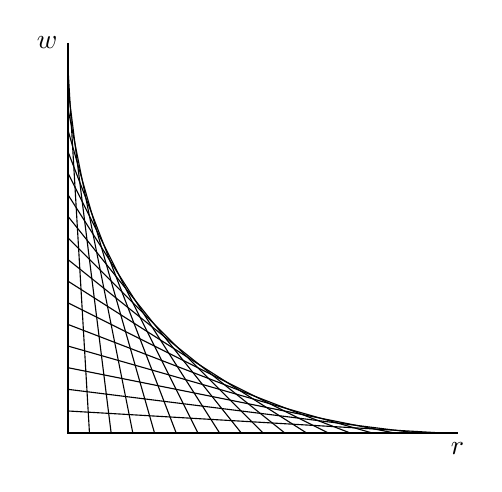
\begin{tikzpicture}[scale=0.55]
		\draw [thick] (0,9) node[left]{\(w\)} -- (0,0) -- (9,0) node[below]{\(r\)};
		\draw (0.5,0) -- (0,8.5);
		\draw (1,0) -- (0,8);
		\draw (1.5,0) -- (0,7.5);
		\draw (2,0) -- (0,7);
		\draw (2.5,0) -- (0,6.5);
		\draw (3,0) -- (0,6);
		\draw (3.5,0) -- (0,5.5);
		\draw (4,0) -- (0,5);
		\draw (4.5,0) -- (0,4.5);
		\draw (5,0) -- (0,4);
		\draw (5.5,0) -- (0,3.5);
		\draw (6,0) -- (0,3);
		\draw (6.5,0) -- (0,2.5);
		\draw (7,0) -- (0,2);
		\draw (7.5,0) -- (0,1.5);
		\draw (8,0) -- (0,1);
		\draw (8.5,0) -- (0,0.5);
	\end{tikzpicture}
\end{figure}
\subsection{Reswitching or ``double-switching'' of techniques}
	\begin{itemize}
		\item As \( r \) rises from below \( r_1 \) to above \( r_1 \Rightarrow \) a switch from technique \( \gamma \) to technique \( \varepsilon \)
		\item As \( r \) rises from below \( r_2 \) to above to above \( r_2 \Rightarrow \) a switch back to technique \( \gamma \)
		\item \( \Rightarrow \) “reswitching''
	\end{itemize}
	\begin{figure}[H]
		\centering
		\begin{tikzpicture}[scale=0.55]
			\draw [thick, dashed, color=myred] (0,7.5) -- (2.6,5.8);
			\draw [thick, dashed, color=myred] (0,7.5) -- (5.75,2.7);
			\draw [thick, dashed, color=mygreen] (0,6.5) -- (2.6,5.8);
			\draw [thick, dashed, color=mygreen] (0,6.5) -- (5.75,2.7);
			\draw [dash dot] (2.6,0) node[below]{\( r_1 \)} -- (2.6,5.8) node[above right]{\( A \)};
			\draw [dash dot] (5.75,0) node[below]{\( r_2 \)} -- (5.75,2.7) node[above right]{\( B \)};
			\draw [thick,color=myblue] (0,7.5) node[left,color=black]{\(q_\gamma\)} to [in=120,out=-30] (7.5,0);
			\draw [thick] (0,6.5) node[left]{\(q_\varepsilon\)} to [in=95,out=-5] (6.5,0);
			\filldraw[black] (2.6,5.8) circle (3pt);
			\filldraw[black] (5.75,2.7) circle (3pt);
			\draw[<-] (2,6.5) -- (2.5,8) node[above]{\( w(r)_\gamma \)};
			\draw[<-] (5,4.5) -- (5.5,6) node[above]{\( w(r)_\varepsilon \)};
			\draw [thick] (0,9) node[left]{\(w\)} -- (0,0) -- (9,0) node[below]{\(r\)};
		\end{tikzpicture}
	\end{figure}
	\begin{itemize}
		\item Reswitching \( \Rightarrow \) problems for the notion that one can unambiguously order techniques in terms of capital-intensity 
		\item i.e. profitability of techniques could not be ranked in a monotonic way in relation to the rate of interest
		\item But if techniques were associated with specific levels of capital-intensity \( \Rightarrow \) also that capital intensity could not be ranked in a monotonic way with the rate of interest
		\item i.e. if techniques \( \varepsilon \) and \( \gamma \) represented given levels of capital-intensity and as \( r \) fell,  techniques switched from \( \gamma \) to \( \varepsilon \) and back to \( \gamma \), the relation between capital intensity and \( r \) could not be monotonic 
		\item Discovered that non-monotonic behaviour could occur independently of reswitching
		\item  “Two-economies [exactly alike] experiencing steady-state growth, could be employing exactly the same technique although in one the rate of profit could be relatively low … while in the other the rate of profit would be relatively high'' (Jones, 1975, p.140)		
	\end{itemize}
	\begin{figure}[H]
		\centering
		\begin{tikzpicture}[scale=0.55]
			\draw [thick,color=myred] (0,8) to [in=-200,out=-70] (8,0);
			\draw [thick,color=myblue] (0,6.5) -- (6.5,0);
			\filldraw[black] (1.3,5.2) circle (3pt);
			\draw [dash dot] (0,5.2) -- (1.3,5.2);
			\draw [dash dot] (1.3,0) node[below]{\( r_1 \)} -- (1.3,5.2);
			\filldraw[black] (5.2,1.3) circle (3pt);
			\draw [dash dot] (0,1.3) -- (5.2,1.3);
			\draw [dash dot] (5.2,0) node[below]{\( r_2 \)} -- (5.2,1.3);
			\node at (3,4) [color=myblue,node font=\boldmath] {\( \alpha \)};
			\node at (6.5,1.2) [color=myred,node font=\boldmath] {\( \beta \)};
			\draw [thick] (0,9) node[left]{\(w\)} -- (0,0) -- (9,0) node[below]{\(r\)};
		\end{tikzpicture}
	\end{figure}
\subsection{Reverse capital deepening}
	\begin{itemize}
		\item ``Reverse capital deepening'' \( \Rightarrow \) increase in the value of capital per worker as \( r \) rises from below \( r_2 \) to above to above \( r_2 \). 
	\end{itemize}
	\begin{figure}[H]
		\centering
		\begin{tikzpicture}[scale=0.55]
			\draw [thick, dashed, color=myred] (0,7.5) -- (2.6,5.8);
			\draw [thick, dashed, color=myred] (0,7.5) -- (5.75,2.7);
			\draw [thick, dashed, color=mygreen] (0,6.5) -- (2.6,5.8);
			\draw [thick, dashed, color=mygreen] (0,6.5) -- (5.75,2.7);
			\draw [dash dot] (2.6,0) node[below]{\( r_1 \)} -- (2.6,5.8) node[above right]{\( A \)};
			\draw [dash dot] (5.75,0) node[below]{\( r_2 \)} -- (5.75,2.7) node[above right]{\( B \)};
			\draw [thick,color=myblue] (0,7.5) node[left,color=black]{\(q_\gamma\)} to [in=120,out=-30] (7.5,0);
			\draw [thick] (0,6.5) node[left]{\(q_\varepsilon\)} to [in=95,out=-5] (6.5,0);
			\filldraw[black] (2.6,5.8) circle (3pt);
			\filldraw[black] (5.75,2.7) circle (3pt);
			\draw[<-] (2,6.5) -- (2.5,8) node[above]{\( w(r)_\gamma \)};
			\draw[<-] (5,4.5) -- (5.5,6) node[above]{\( w(r)_\varepsilon \)};
			\draw [thick] (0,9) node[left]{\(w\)} -- (0,0) -- (9,0) node[below]{\(r\)};
		\end{tikzpicture}
	\end{figure}
\subsection{Reswitching and reverse capital deepening}
	\begin{itemize}
		\item At \( r_1k_\alpha > k_\delta \rightarrow k \) falls with an increase in \( r \) in the vicinity of \( r_1 \)
		\item At \( r_2k_\beta > k_\delta \rightarrow k \) falls with an increase in \( r \)
		\item Reswitching at \( r_3 \) and a rising \( k \)
		\item In fact, it was shown that non-monotonic behaviour could occur without reswitching
		\item i.e. reverse capital deepening (RCD) could occur independently of rewswitching
		\item Significance of RCD?
		\[
		\uparrow r \Rightarrow\uparrow k \Rightarrow \uparrow\frac{\text{V of K}}{L}
		\]
		\item Since \( w \) and \( r \) are inversely related,
		\begin{gather*}
			\Rightarrow\:\downarrow w \text{ with } \uparrow \frac{\text{V of K}}{L}\\
			\Rightarrow\:\downarrow w \text{ with } \downarrow \frac{L}{\text{V of K}}
		\end{gather*}
		For a given endowment of capital in value terms \( \downarrow w \) with \( \downarrow L \)
	\end{itemize}
	\begin{figure}[H]
		\centering
		\begin{tikzpicture}[scale=0.55]
			\draw (2,3.3) -- (2,0) node[below]{\(r_1\)};
			\draw (4,2.6) -- (4,0) node[below]{\(r_2\)};
			\draw (6,1.5) -- (6,0) node[below]{\(r_3\)};
			\draw [smooth,thick,color=myred] plot coordinates {(0,6)(0.3,4.9)(1,4)(2,3.3)(2.8,2.75)(4,2.2)(6,1.5)(8,0)};
			\draw [smooth,thick,color=mygreen] plot coordinates {(0,5.2)(0.3,4.3)(0.75,3.6)(2,3)(4,2.6)(5,2.25)(6,1.5)(6.6,0.85)(7,0)};
			\draw [smooth,thick,color=myblue] plot coordinates {(0,4.25)(0.7,3.75)(1.25,3.5)(2,3.3)(3,3)(4,2.6)(4.8,1.9)(6,0)};
			\draw [line join=round,thick,smooth,color=mygold] {(0,-3.5) -- (2,-3) -- (2,-2)} -- plot coordinates {(2,-2)(3,-2.1)(4,-2)} -- (4,-2.5) -- plot coordinates {(4,-2.5)(4.4,-2.4)(6,-2.75)} -- (6,-3) -- plot coordinates{(6,-3)(7,-3.1)(8,-3.05)};
			\draw [<-] (1,-3.4) -- (1,-4.5) node[below,color=myred,node font=\boldmath]{\(\alpha\)};
			\draw [<-] (3,-2.2) -- (3,-4.5) node[below,color=myblue,node font=\boldmath]{\(\gamma\)};
			\draw [<-] (5,-2.6) -- (5,-4.5) node[below,color=mygreen,node font=\boldmath]{\(\beta\)};
			\draw [<-] (7,-3.2) -- (7,-4.5) node[below,color=myred,node font=\boldmath]{\(\alpha\)};
			\draw [<-] (7.5,-4.8) -- (8.5,-4.8) node[right]{dominant technique is};
			\draw [thick] (0,9) node[left]{\(w\)} -- (0,-4) node[left]{\(k\)};
			\draw [thick] (0,0) node[left]{\(0\)}-- (9,0) node[below]{\(r\)};
		\end{tikzpicture}
	\end{figure}
\subsection{Reverse Capital Deepening and the Orthodox Explanation of Distribution}
	\begin{figure}[H]
		\centering
		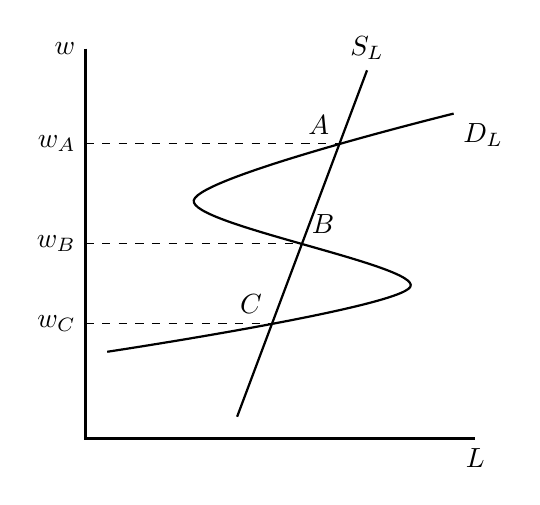
\begin{tikzpicture}[scale=0.55]
			\draw [thick] (3.5,0.5) -- (6.5,8.5) node [above]{\( S_L \)};
			\draw [dashed] (0,2.65) node [left]{\( w_C \)} -- (4.3,2.65) node [above left]{\( C \)};
			\draw [dashed] (0,4.5) node [left]{\( w_B \)} -- (5,4.5) node [above right]{\( B \)};
			\draw [dashed] (0,6.8) node [left]{\( w_A \)} -- (5.85,6.8) node [above left]{\( A \)};
			\draw [thick] (0,9) node[left]{\(w\)} -- (0,0) -- (9,0) node[below]{\(L\)};
			\draw [smooth,thick] plot coordinates {(0.5,2)(7.5,3.5)(2.5,5.5)(8.5,7.5)};
			\node at (8.5,7.5) [below right] {\( D_L \)};
		\end{tikzpicture}
	\end{figure}
	\begin{itemize}
		\item Equilibria A and C are unstable; equilibrium B is stable
		\item \( \Rightarrow \) w's above \( w_A \) would yield upward pressure on \( w \);
		\item \( \Rightarrow \) market would not correct excess \( D_L \)
		\item w's below \( w_C \) would yield downward pressure on w
		\item \( \Rightarrow \) market would not correct excess \( S_L \)
		\item \( \Rightarrow \) would not correct unemployment
		\item In respect of the rate of profit or rental rate on capital, analogous difficulties arise with explanations based on supposed well-behaved factor substitution
	\end{itemize}
	\begin{figure}[H]
		\centering
		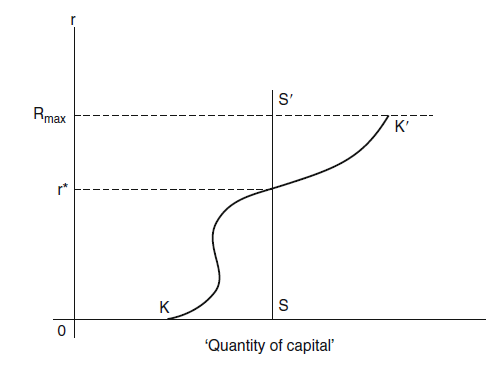
\includegraphics{Figure3}
	\end{figure}
	\begin{itemize}
		\item RCD \( \Rightarrow \) possibility of a positively sloped demand for capital (stock)
		\item RCD also carries worrying implications for the traditional Wicksellian story	   
	\end{itemize}
	\begin{figure}[H]
		\centering
		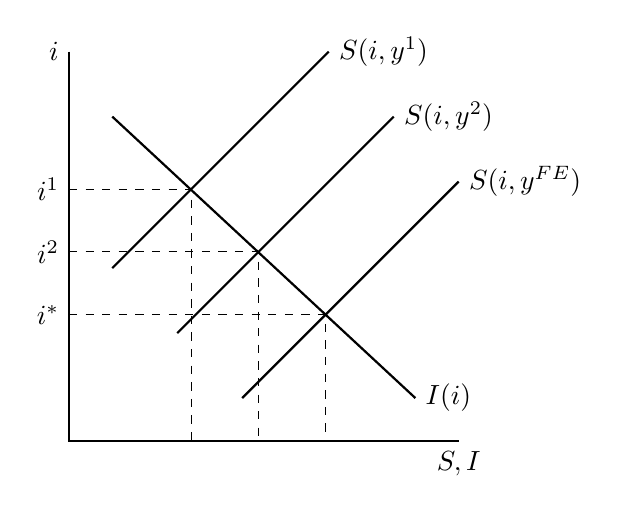
\begin{tikzpicture}[scale=0.55]
			\draw[thick] (0,9) node[left]{\( i \)} -- (0,0) -- (9,0) node[below]{\( S, I \)};
			\draw [thick] (1,7.5) -- (8,1) node[right]{\(I(i)\)};
			\draw [thick] (1,4) -- (6,9) node[right]{\( S(i,y^1) \)};
			\draw [thick] (2.5,2.5) -- (7.5,7.5) node[right]{\( S(i,y^2) \)};
			\draw [thick] (4,1) -- (9,6) node[right]{\( S(i,y^{FE}) \)};
			\draw [dashed] (0,5.825) node[left]{\( i^1 \)} -- (2.825,5.825) -- (2.825,0);
			\draw [dashed] (0,4.375) node[left]{\( i^2 \)} -- (4.375,4.375) -- (4.375,0);
			\draw [dashed] (0,2.925) node[left]{\( i^* \)} -- (5.925,2.925) -- (5.925,0);
		\end{tikzpicture}
		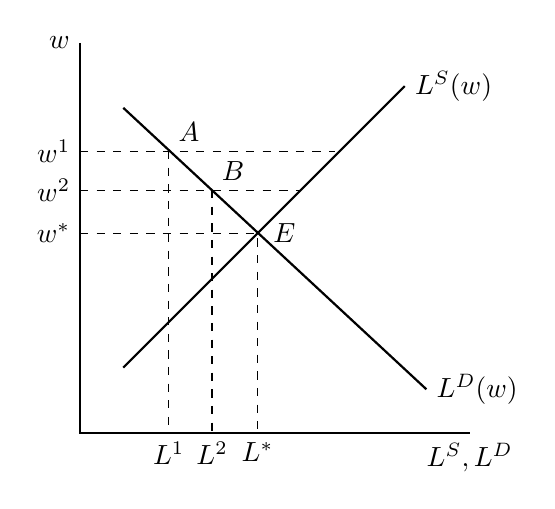
\begin{tikzpicture}[scale=0.55]
			\draw[thick] (0,9) node[left]{\( w \)} -- (0,0) -- (9,0) node[below]{\( L^S,L^D \)};
			\draw [thick] (1,7.5) -- (8,1) node[right]{\( L^D(w) \)};
			\draw [thick] (1,1.5) -- (7.5,8) node[right]{\( L^S(w) \)};
			\draw [dashed] (0,6.5) node[left]{\( w^1 \)} -- (5.9,6.5);
			\draw [dashed] (2.05,6.5) node[above right]{\( A \)} -- (2.05,0) node[below]{\(L^1\)};
			\draw [dashed] (0,5.6) node[left]{\( w^2 \)} -- (5.1,5.6);
			\draw [dashed] (3.05,5.6) node[above right]{\( B \)} -- (3.05,0) node[below]{\(L^2\)};
			\draw [dashed] (0,4.6) node[left]{\( w^* \)} -- (4.1,4.6) node[right]{\( \: E \)} -- (4.1,0) node[below]{\(L^*\)};
		\end{tikzpicture}
	\end{figure}
	\begin{itemize}
		\item To the extent that the traditional explanation of the rate of interest rests on the decreasing investment demand function and this in turn rests on the notion that a fall in r entails a rise in the capital to labour ratio, then this explanation is open to doubt via the results of the capital-theoretic critique
		\item \( \Rightarrow \) reverse capital deepening would call into question the stability of the \textit{S-I} equilibrium in the traditional Wicksellian story
		\item \( \Rightarrow \) raises questions about the existence of a mechanism ensuring investment would adapt to the full-employment level of saving
	\end{itemize}

\section{Demand-Constrained Approaches to the Theory of Output and Growth}
\subsection{The Basis for a Non-Marginalist Theory of Output}
	\begin{itemize}
		\item  Capital-theoretic critique of the orthodox appoach to value and distribution \( \Rightarrow \) simultaneously a critique of the traditional theory of output
		\item Recall this critique shows \textit{inter alia} that outside of a one-commodity world one cannot assert a monotonic relation between relative factor returrns and relative factor proportions
		\item \( \Rightarrow \) removes traditional theoretical ground from inverse investment - interest rate relation (as well as real wage - labour demand relation)
		\item But this is not only a critique of the Wicksellian theory of the rate of interest
		\item It also weakens traditional orthodox arguments (which Keynes does not dispatch) by which wage and price flexibility would push effective demand to a level consistent with full-employment
		\item Weakens the basis for the conventional belief that the aggregate demand function is monotonically inverse and thus that the LRAS is vertical at FE
		\item  Including newer justifcations such as the New Keynesian AD curve (White, CJE, 2015)
		\item Simultaneously this critique removes some of the problematic aspects of Keynes's own critique of orthodoxy and puts his alternative theory on firmer ground
		\item That alternative \( \Rightarrow \) \textit{the principle of effective demand}
		\begin{itemize}
			\item investment governs saving
			\item no spontaneous tendency towards full-employment
			\item demand-deficient unemployment is not peculiar to the ``short-run'' or a world of rigidities / imperfections
		\end{itemize}
	\end{itemize}
\subsubsection{Kalecki and Keynes}
	\begin{itemize}
		\item Contemporaneously with Keynes, Michal Kalecki had arrived at similar conclusions
		\item ``\textit{An Essay on the Theory of the Business Cycle}'' published in 1933, anticipated some results set out by Keynes in 1936
		\item Though Kalecki's argument was set out in the context of the business cycle and derived from a study of Marx (interesting Introduction by Joan Robinson to \textit{Kalecki's Studies in the Theory of Business Cycles}, 1962)
		\item Kalecki's (1933) formulation for a closed economy with no government can be arrived at by supposing income consists solely of wages and profits and that all wages are spent
		\item For equilibrium
		\begin{equation}
			Y = C_w + B_0 + \lambda P + A = W + B_0 + \lambda P + A \label{E:4.1}
		\end{equation}
		\item Suppose the distribution of income is such that
		\begin{equation}
			P = \pi_y Y \Rightarrow Y = W + P \label{E:4.2}
		\end{equation}
		\item Hence
		\begin{equation}
			W = \frac{1-\pi_y}{\pi_y} P \label{E:4.3}
		\end{equation}
		\item In turn
		\begin{equation}
			\frac{P}{\pi_y} = \frac{1-\pi_y}{\pi_y}P+B_0+ \lambda P + A \label{E:4.4}
		\end{equation}
		\item and thus
		\begin{equation}
			P = \frac{B_0+A}{1-\lambda} \label{E:4.5}
		\end{equation}
		\item Thus the profit flow to capitalists is a multiple of the sum of the ``constant part of capitalists' consumption, and \dots\: the gross accumulation which is equal to the production of investment goods'' (Kalecki, 1933, 1962)
		\item The source of Kalecki's famous remark:
		\begin{quote}
			``The workers spend what they get: the capitalists get what they spend''
		\end{quote}
		\item Important to note that \cref{E:4.5} implies that with the ``constant'' part of capitalists' consumption given, the flow of saving (in this simple case, equal to the flow of profit) is governed by ``gross accumulation'' i.e. by investment\
		\item Kalecki's discovery of the principle of effective demand couched in terms of the dynamics of profit and investment
		\item And underpinned by a theory of distribution whereby the mark-up and thus share of profit income was a reflection of the ``degree of monopoly''
		\item Some debate over the last 30-40 yrs in heterodox circles (Sraffians vs Kaleckians) over this approach to relative prices and distribution as representing an alternative to a marginalist approach
	\end{itemize}
\subsection{A Non-Marginalist Approach to Output, Value and Distribution}
	\begin{itemize}
		\item A critical question for heterodoxy since the 1950's: what are contours of the alternative theory founded on a both a non-marginalist theory of output and a non-marginalist theory of value and distribution?
		\item Response to this has adopted either Kalecki's or Keynes's approach to the development of an alternative theory of output
		\item Specifically one centered on the principle of effective demand and which eschews a traditional marginal productivity approach to distribution
		\item Two main lines of development:
		\begin{enumerate}[label=\textbf{\arabic*.}]
			\item Inspired by both Keynes and Kalecki, an extension of the principle of effective demand to the long-run, where changes in distribution play a critical role in the long-run adjustment of saving to investment
			\begin{itemize}
				\item Earliest iteration labelled Cambridge or Post-Keynesian embodied in the non-orthodox growth theory of the 1950's -- 1970's
				\item Developed into modern Kaleckian/neo-Kaleckian growth models
			\end{itemize}
			\item Comparatively more recent -- starting in the mid-1980's -- a reconsideration of Keynes's version of the principle of effective demand for a long-run setting fused with a modern-classical inspired explanation of relative prices and distribution
			\begin{itemize}
				\item The latter approach is sometimes labelled ``Sraffian''; since the inspiration for the accompanying explanation of relative prices and distribution is primarily the work of Sraffa (1960)
				\item At various points since the 1980's some tension between these two approaches
				\item Will deal with this tension later
			\end{itemize}
		\end{enumerate}
	\end{itemize}
\subsection{Growth and Distribution}
\subsubsection{Cambridge / post-Keynesian Theory}
	\begin{itemize}
		\item In part a reaction to the growth theory of Solow and Swan in the mid-1950's
		\item In part an attempt to extend the notion of effective demand to the long-run (hence necessarily a growth setting)
		\item In part a response to deficiencies in the traditional explanation of distribution
		\item In part inspired by the fusion of discussion about output and about distribution of Kalecki
	\end{itemize}
\subsubsection{Robinson and Kaldor on Saving, Distribution and Accumulation}
	\begin{itemize}
		\item With income splitting into wages and profits only, aggregate saving is given by 
		\begin{equation}
			S = s_c P + s_w W \Rightarrow \frac{S}{Y}=s=s_c \frac{P}{Y}+s_w\frac{W}{Y} \label{E:4.6}
		\end{equation}
		\item Since
		\begin{equation}
			Y = P + W \label{E:4.7}
		\end{equation}
		\begin{align}
			\frac{S}{Y} = s &= s_c \frac{P}{Y} + s_w\frac{(Y-P)}{Y} = s_c \frac{P}{Y} + s_w - s_w\frac{P}{Y} \\\notag
			&= \left( s_c-s_w \right) \frac{P}{Y} + s_w \label{E:4.8}
		\end{align}
		\begin{equation}
			\therefore \frac{S}{Y} = s = \left( s_c - s_w \right) \frac{P}{Y} + s_w \label{E:4.9}
		\end{equation}
		\item \textbf{\( \Rightarrow \) even with given \( s_c \) and \( s_w \), aggregate \( s \) varies with P/Y}
		\item In equilibrium
		\begin{equation}
			\frac{I}{Y} = \frac{S}{Y} = s = \left( s_c - s_w \right) \frac{P}{Y} + s_w \label{E:4.10}
		\end{equation}
		\begin{equation}
			\therefore \frac{P}{Y} = \frac{1}{\left( s_c - s_w \right)}\frac{I}{Y}-\frac{s_w}{\left( s_c - s_w \right)} \label{E:4.11}
		\end{equation}
		\item A given capital to output ratio \( \Rightarrow \) share of investment in output depends on the rate of accumulation
		\begin{equation}
			\frac{I}{Y} = \frac{I}{K}\frac{K}{Y} = g_k v \label{E:4.12}
		\end{equation}
		\begin{equation}
			\therefore \frac{P}{Y} = \frac{1}{\left( s_c - s_w \right)}g_k v - \frac{s_w}{\left( s_c - s_w \right)} \label{E:4.13}
		\end{equation}
		\item With \( s_w = 0 \),
		\begin{equation}
			\frac{P}{Y} = \frac{1}{s_c} g_k v = \frac{1}{s_c} g_k \frac{K}{Y} \label{E:4.14}
		\end{equation}
		\item From \cref{E:4.14} one can derive a relation between the equilibrium growth, capitalists' propensity to consume and the rate of profit:
		\begin{equation}
			\frac{P}{Y}\frac{Y}{K} = \frac{1}{s_c}g
			\quad \text{and} \quad
			\frac{P}{Y}\frac{Y}{K} = \frac{P}{K} = r \label{E:4.15}
		\end{equation}
		\item The Cambridge growth equation
		\begin{align}
			r &=  \frac{1}{s_c}g \notag\\
			s_c r &= g \label{E:4.16}
		\end{align}
	\end{itemize}
\subsubsection{The Composition of Aggregate Demand and the Distribution of Income}
	\begin{itemize}
		\item 2-sector case: consumption-good, investment good;
		\item Labour and capital good are inputs in both sectors.
		\item Assume all wages are spent and all profit saved
		\item Assume output is equal to demand (equilibrium)
		\begin{equation}
			p_c Y_c = C = w_m \left( L_c + L_i \right) \Rightarrow \frac{w_m}{p_c} = \frac{Y_c}{\left( L_c + L_i \right)} \label{E:4.17}
		\end{equation}
		\item With \( Y_c = L_c \frac{Y_c}{L_c} \), then
		\begin{equation}
			\frac{w_m}{p_c} = \frac{L_c}{\left( L_c + L_i \right)}\frac{Y_c}{L_c} \label{E:4.18}
		\end{equation}
		\item \(\Rightarrow\) real wage is in a definite relation with the composition of demand, given \( \frac{Y_c}{L_c} \)
		\item  Profits in the consumption good sector can be related to activity in the investment good sector: 
		\begin{equation}
			\Pi_c = p_c Y_c - w_m L_c = w_m L_c + w_m L_i - w_m L_c \label{E:4.19}
		\end{equation}
		\item \( \Rightarrow \) profits of the consumption-good sector are determined by the wage bill of the investment good sector
		\item With output equal to demand in the investment-good sector
		\begin{equation}
			p_i Y_i = p_i \left( I_i + I_c \right) = w_m L_i + \Pi_i = \Pi_c + \Pi_i \label{E:4.20}
		\end{equation}
		\item \( \Rightarrow \) aggregate profits are ``governed'' by aggregate investment 
		\item Assume an increase in the growth rate of investment relative to consumption demand
		\item \( \Rightarrow \) demand for consumption good increases relative to output of the consumption good \( \Rightarrow \) rise in prices relative to money wage
		\item Comparison of two economies alike except for level of \textit{I} \( \rightarrow \) smaller real wage and higher profit flow and in economy with larger \textit{I}
		\item \textcolor{myred}{\( \Rightarrow \) and a higher \textit{I} relative to \textit{K} (i.e. faster growth) \( \Rightarrow \) a higher profit flow relative to \textit{K} \( \Rightarrow \) a higher rate of profit, \textit{r}}
	\end{itemize}
\subsubsection{The Cambridge Equation as a Theory of Distribution and Long-Run Counterpart to Keynes's PED}
	\begin{itemize}
		\item The Robinson-Kaldor connection in terms of the Cambridge equation was ``corrected'' in the 1960's by Pasinetti
		\item Demonstrated that \cref{E:4.16} held even when allowing for workers' saving i.e \( s_w \neq 0 \)
		\item In other words, the relation between the rate of growth and the rate of profit is independent of the propensity to save of workers
		\item Source of this result was that workers would receive profit in proportion to their saving:
		\begin{quote}
			``In the long-run, when workers save, they receive an amount of profits such as to make their total savings exactly equal to the amount that capitalists would have saved out of workers' profits if these profits remained to them'' (Pasinetti, 1974, p.111)
		\end{quote}
			\item General interpretation of the Cambridge equation as a theory of distribution
		\item And as a long-run counterpart of Keynes's principle of effective demand
		\item i.e. in Keynes (formally) output and employment fluctuate to bring \textit{S} into line with \textit{I} -- this involves fluctuation in capacity utilisation
		\item Cambridge approach provided for a change in distribution to adapt \textit{S} to \textit{I} in the long-run
		\item Kaldor (1955-56) arguing that this was the Keynesian adjustment for a growing economy 
		\item For both Robinson and Kaldor -- as noted already -- aggregate saving would change with changes in the distribution of income
		\item Coupled with the rejection of marginal productivity theory, the notion that changes in the growth rate could generate changes in \textit{w} and \textit{r} \( \Rightarrow \) and adjustments in \textit{S/K} in line with \textit{I/K}
	\end{itemize}
\subsubsection{Dispute over the Equation and the Appropriate Characterisation of Long-Run Effective Demand}
	\begin{itemize}
		\item By early 1980's debate opening up over the appropriate interpretation of the Cambridge equation
		\item And by implication, over the mechanics by which \textit{S} adapts to \textit{I} in the long-run
		\item Some tension between the Cambridge approach and those following a Sraffian approach
		\item From a Sraffian (modern classical approach) \(g = s_cr\)  could not be interpreted as referring to the `normal' `r' and be consistent with the \textit{PED}
		\item Argument by Garegnani, Kurz early -- mid 1980's: if \textit{r} refers to the normal rate of profit and thus the underlying utilisation is the normal rate -- i.e. the rate (presumably cost-minimising) anticipated on average for capacity when investment decisions are beng made
		\item But then `\textit{g}' could not be the actual or realised rate of accumulation (growth)
		\item Otherwise this would imply an actual growth generating normal utilisation and thus demand conforming to capacity; and \textit{S} driving \textit{I}
	\end{itemize}
	\begin{align*}
		g &= \frac{I}{K} = \frac{Y_i}{K_i}\frac{K_i}{K}\\
		g &= \frac{I}{K} = \frac{Y_i}{Y_i^F}\frac{Y_i^F}{K_i}\frac{K_i}{K}\\
		u_i &= \frac{Y_i}{Y_i^F}\\
		g &= \frac{I}{K} = u_i \frac{Y_i^F}{K_i}\frac{K_i}{K}
	\end{align*}
	\begin{itemize}
		\item From this perspective, interpreting `\textit{r}' as the normal rate of profit -- and thus the rate to be explained by a theory of distribution would be ``un-Keynesian''
		\item And thus if `\textit{g}' refers to the realized growth rate, then `\textit{r}' must refer to the realized rate of profit as distinct from the normal rate
		\item This Sraffian position rejects the notion that distributional changes in the long-run are necessary to bring saving into line with investment
		\item Distributional changes are not necessary for this adjustment (Garegnani, 1992)
		\item Rather (Garegnani, 1992), output and income changes which adjust \textit{S} to \textit{I} in the long can be facilitated through changes in the scale of capacity
		\item In a cyclically-disturbed system, average and normal utilisation are typically less than 100\%
		\item This provides the elasticity for the system to respond to an increasing rate of growth of demand via an increasing growth rate of the capital stock and hence productive capacity
		\item Alternative positions adopted within the ``non-Sraffian'' / Kaleckian camps was to stress that the modern classical approach, with \textit{r} determined independently of \textit{s} and \textit{g} did indeed suggest that a \textit{S/K} generated a higher \textit{I/K} and hence the Sraffian approach was inconsistent with the primacy of effective demand in the long-run
		\item Sraffians reject this
		\item Some Kaleckians argued against the Sraffian position on methodological grounds
		\item The next stage in this debate was really initiated by modern Kaleckian reformulations of the post-Keynesian growth model
	\end{itemize}
\subsubsection{Modern Post-Keynesian/Kaleckian Models}
	\begin{itemize}
		\item Modern Kaleckian theorists take `\( g \)' as endogenous, by combining the Cambridge Growth \cref{E:4.16} with an explanation of the rate of accumulation
		\item From Blecker (2002)
		\begin{equation}
			p = wl\varphi \quad\text{with}\quad \varphi>1 \label{E:4.21}
		\end{equation}
		\item Profit share \( \pi \) is given by
		\begin{equation}
			\pi = \frac{p-wl}{p} = 1-\frac{w}{p}l = \frac{\varphi-1}{\varphi} \label{E:4.22}
		\end{equation}
		\item Profit rate \( r \) is given by
		\begin{equation}
			r=\left(\frac{p-wl}{p}\right)\frac{Y}{K} = \left( \frac{\varphi-1}{\varphi} \right) u = \pi u \label{E:4.23}
		\end{equation}
		\item The rate of accumulation which would absorb exactly the flow of savings is
		\begin{equation}
			g^s - s_c r \left( =\frac{S}{\pi}\frac{\Pi}{K} \right) \label{E:4.24}
		\end{equation}
		\item On the basis of an investment function like
		\begin{equation}
			I_t = A + \alpha\Pi_t + \beta Y_t - \gamma K_t \label{E:4.25}
		\end{equation}
		one can write (dividing throigh by K) a ``desired accumulation'' function in the form
		\begin{equation}
			g^i = f_0 + f_1r + f_2u_t \label{E:4.26}
		\end{equation}
		\item For equilbrium growth \( g^s = g^i \)
		\begin{equation}
			\Rightarrow \frac{S}{K}=\frac{I}{K} \quad\text{and therefore}\quad s_c r = f_0+f_1r+f_2 u_t \label{E:4.27}
		\end{equation}
		\item Substituting \( \pi u \) for \( r \) in \cref{E:4.27} gives
		\begin{equation}
			s_c\pi u = f_0 + f_1 \pi u + f_2 u \label{E:4.28}
		\end{equation}
		\item and therefore steady-state \( u \) is given by
		\begin{equation}
			u^*=\frac{f_0}{(s_c - f_1)\pi - f_2} \label{E:4.29}
		\end{equation}
		\item Stability of steady state growth requires saving to react to changes in utilisation more than investment
		\item \( \uparrow s_c \) leads to a fall in \( g^*, u^* \) and \( r^* \Rightarrow \) ``paradox of thrift''
	\end{itemize}
	\begin{figure}[H]
		\centering
		\begin{tikzpicture}[scale=0.55]
			\draw [thick,color=myblue] (0,3) -- (8,8) node [above right] {\( f_0+f_1\pi u + f_2 u \)};
			\draw [thick,dashed,color=myred] (0,0) -- (4,9) node [above] {\( s_c^i\pi u \)};
			\draw [thick,dashed, color=mygreen] (0,0) -- (7,9) node [above] {\( s_c\pi u \)};
			\draw [dashed] (0,4.15) node [left] {\( g^{*'} \)} -- (1.85,4.15) -- (1.85,0) node [below] {\( u^{*/} \)};
			\draw [dashed] (0,5.85) node [left] {\( g^{*} \)} -- (4.5,5.85) -- (4.5,0) node [below] {\( u^{*} \)};
			\draw [thick] (0,9) node [above]{\( g \)} -- (0,0) -- (9,0) node [right]{\( u \)};
		\end{tikzpicture}
	\end{figure}
	\begin{itemize}
		\item In this model a (assuming a stable \( g^* \)) shift in distribution towards profit reduces utilisation, the profit rate and \( g^* \) - referred to as the ``stagnationist'' case
		\item This case has non-orthodox implications about the relation between the real wage and employment. From \cref{E:4.29}
		\begin{equation}
			\frac{du^*}{d\pi} = \frac{-(s_c-f_1)f_0}{[(s_c-f_1)\pi-f_2]^2} \label{E:4.30}
		\end{equation}
		\item Since, for stability, \( f_1,\pi + f_2 \leq s_c\pi \), and thus \( \frac{f_2}{\pi} < (s_c-f_1) \), then, with \( f_2 \) and \( \pi > 0 \), \( (s_c-f_1) > 0 \) and thus \( \frac{du^*}{d\pi} < 0 \)
		\item In turn, since
		\begin{equation}
			I = \frac{L}{Y}\frac{Y}{K}K=l\cdot u \cdot K \label{E:4.31}
		\end{equation}
		\item \( \Rightarrow L \)  per unit of \( K \) rises with utilisation, and thus with a fall in \( \pi \) and thus with a \textbf{rise} in the real wage \( \frac{w}{P} \)
		\item This case also suggests a positive relation between the steady state rate of profit and the real wage 
		\item i.e. a fall in the profit share -- rise in the real wage -- increases aggregate demand, utilisation and accumulation
		\item The increase in utilisation outweighs effect of a fall in \( \pi \) on the rate of profit, \( r \),  so that \( r \) rises
		\item Subsequent debate suggested that the simple model above exaggerated the effects of changes in utilisation rates \( (u) \) on investment demand (\cref{E:4.28}) 
		\item A more general alternative suggested for the desired accumulation function was
		\begin{equation}
			g^i = h(\pi,u) \quad h_{\pi},h_u>0 \label{E:4.32}
		\end{equation}
		\item \( \Rightarrow \) an increase in profit share, for a given utilisation and an increase in utilisation for a given profit share would both increase the desired rate of accumulation
		\item  Steady state utilisation rate is the solution to
		\begin{equation}
			s_c\pi u = h(\pi,u) \quad\text{with}\quad \frac{du}{d\pi} = \frac{-\left( s_cu-h_{\pi} \right)}{s_c\pi-h_u} \label{E:4.33}
		\end{equation}
		\item Stability of the steady state requires
		\[
			s_c\pi-h_u>0
		\]
		\item Whether `\( u^* \)' rises or falls with a rise in the profit share turns on whether \( s_c u-h_{\pi} \) is < 0 or > 0
		\item If \( s_c u-h_{\pi} > 0, \frac{du}{d\pi}<0 \Rightarrow \) ``stagnationist'' case
		\item Although a rise in the profit share, \( \pi \), has a positive effect, \textit{ceteris paribus}, on the desired rate of accumulation (and potentially on \( u \)), there is a greater negative effect on utilisation (via the fall in the real wage depressing consumption demand)
		\item \( \Rightarrow \) negative impact on the steady state rate of accumulation and on the steady state rate of profit
		\item Alternative possibility, referred to in the literature as the ``exhilarationist'' case
		\item Suppose that \( s_c\pi-h_u<0 \), then \( \frac{du}{d\pi}>0 \)
		\item \( \Rightarrow \) a redistribution of income towards profits has a net stimulatory effect on aggregate demand
		\item \( \Rightarrow \) stimulus to utilisation via the positive effect of a rise in \( \pi \) on capitalists' consumption and accumulation outweighs negative impact on utilisation from a falling real wage reducing workers' consumption
		\item The steady state rate of accumulation and the steady state rate of profit both rise
		\item These different cases entail two different relations between steady state distribution and the steady state
		\item The stagnationist case: a rise in \( g^* \), a fall in the \( \pi \) and \underline{a rise in the real wage}, steady state utilisation \underline{and rate of profit}
		\item The exhilarationist case: a rise in \( g^* \), a rise in \( \pi \), \underline{a fall in the real wage, a rise in the rate of profit} and a rise in steady state utilisation
		\item The ``stagnationist'' case may also be referred to as ``wage-led'' growth while the ``exhilarationist'' case may be referred to as ``profit-led'' growth
		\item As Blecker (2003) notes, there are intermediate cases between the stagnationist and exhilarationist possibilities 
	\end{itemize}
\subsubsection{Kaleckian and Sraffians: Utilisation and Distribution}
	\begin{itemize}
		\item Worth noting two issues on which there has been some disagreement between Kaleckians and Sraffians
		\begin{enumerate}[label=\textbf{\arabic*.}]
			\item Simple model above shows that along with the steady state growth rate, the steady state utilisation rate, \( u^* \), is endogenous
			\begin{itemize}
				\item Earlier Kaleckian models showed that the steady state \( u \) need not correspond to a ``normal'' utilisation rate, \( u_n \)
				\item Problematic to the extent that the ``normal'' rate is to be interpreted as a ``desired'' rate, even as a long-run average
			\end{itemize}
			\item The possibility associated with the ``stagnationist'' case that the rate of profit and real wage move in the same direction is at odds with the Sraffian approach
			\begin{itemize}
				\item Not unrelated to the difference between steady state and ``normal'' utilisation
				\item As well as the methodological differences between the two camps
				\item In recent years -- some attempt at reconciliation (particularly by Lavoie) viz., by including within the Kaleckian approach a mechanism pushing steady state utilisation towards the normal rate over the long-run
			\end{itemize}
		\end{enumerate}
	\end{itemize}
\section{Modern Classical Approaches to Value and Distribution and Demand-Led Growth}
\subsection{Possibilities for a Sraffa-Keynes Synthesis}
	\begin{itemize}
		\item The modern classical approach \( \Rightarrow \) modern reconstruction of CPE associated mainly with Sraffa (1960)
		\item Not only an alternative view of value and distribution but also a critique of marginalist approach
		\item As already noted, that critique strengthens Keynes's Principle of Effective Demand
		\item \( \Rightarrow \) strengthens notion that effective demand can settle at a level consistent with involuntary unemployment even in the presence of wage and price flexibility
		\item Alternatively put, wage/price/interest rate flexibility cannot ensure spontaneous convergence to full-employment
	\end{itemize}
\subsubsection{Complimentarities}
	\begin{itemize}
		\item Sraffa's reconstruction of CPE \( \Rightarrow \) resurrection of ``core'' (à la Garegnani): surplus-based explanation of relative prices and their connection with income distribution
		\item One which leaves output ``open'' -- to the extent that constant returns to scale are assumed
		\item A strengthened principle of effective demand in Keynes -- without the marginalist theory of value \( \Rightarrow \) relative prices and distribution left ``open''
		\item e.g. minus the traditional labour demand curve; minus the investment demand function
		\item Suggests a complimentarity and the possibility of synthesis
		\item The modern classical approach \( \Rightarrow \) the explanation of relative prices and distribution lacking in Keynes; the PED \( \Rightarrow \) an explanation of outputs left open in the modern classical approach
	\end{itemize}
\subsubsection{A Sraffa-Keynes Synthesis}
	\begin{itemize}
		\item Sraffian reconstruction of CPE \( \Rightarrow \) a multi-commodity basis for a theory of output centered around the principle of effective demand (PED)
		\item \( \Rightarrow \) a ``multi-commodity'' view of the PED
		\item \( \Rightarrow \) an alternative ``microfoundations'' and not one wedded to the methodological individualism of conventional economics
		\item Also a more coherent basis for the connection between interest and distribution which Keynes himself had sought
		\item Two important aspects to this synthesis:
		\begin{enumerate}[label=\textbf{\arabic*.}]
			\item How is the principle of effective demand altered in a multi-commodity framework, where relative prices and income distribution are determined as in the modern classical approach?
			\item What is the significance for the principle of effective demand of the fact that one distributive variable is exogenous in the modern classical approach
		\end{enumerate}
		\item Keynesian multiplier will now consist of a number of ``multipliers'' -- one for each commodity output as a function of autonomous demand
		\item e.g. in the two-sector case gross-outputs of commodities 1 and 2 can be written as multiples of autonomous investment demands for commodities 1 and 2 \( \Rightarrow \)
		\begin{align}
			Y_i &= C_i+I_{Ri}+I_i \notag\\
			C_i &= c_{wi}(W+P_w)+c_{ci}P_c\\
			I_{Ri} &= Y_1a_{i1}+Y_2a_{i2} \notag
		\end{align}
		\item Propensities to consume are given by
		\[
			c_{w1} = \frac{C_1^w}{W+P_w} \quad c_{w2}=\frac{p_{21}c_2^w}{W+P_w} \quad c_{c1}=\frac{C_1^c}{Pc} \quad c_{c2}=\frac{p_{21}C_2^c}{P_c}
		\]
		\item \( \Rightarrow \) gross output \( Y \) for both sectors is a function of gross outputs of both sectors as well as autonomous demands \( I_1 \) and \( I_2 \) independent of \( Y \)'s
		\item \( \Rightarrow \) solving for \( Y_1 \) and \( Y_2 \) would yield expressions of the form
		\begin{align}
			Y_1 &= m_{11}I_1 + m_{21}I_2 \notag\\
			Y_2 &= m_{12}I_2 + m_{22}I_2 \notag\\
			\intertext{and}
			\frac{Y_1}{Y_2} &= \frac{m_{11}I_1 + m_{21}I_2}{m_{12}I_2 + m_{22}I_2}
		\end{align}
		\item \( m \)'s are income-expenditure multipliers
		\item \textcolor{myred}{\( \Rightarrow \) multi-commodity version of the income-expenditure multiplier in simple Keynesian model}
		\item In a multi-commodity context output multipliers and therefore employment multipliers depend on relative prices and income distribution
		\item If there is autonomous demand for each commodity \( \Rightarrow \) aggregate employment multiplier depends on ratio of autonomous demands
		\item \( \Rightarrow \) composition of aggregate autonomous demand will most likely influence aggregate employment, if autonomous demand for individual commodities have different output multipliers
		\item Changes in distribution affect output and employment through a number of channels:
		\begin{itemize}
			\item directly affecting \( m \)'s
			\item directly affecting autonomous demands
			\item indirect effects on \( m \)'s via changes in \( a_{ij} \)'s
		\end{itemize}
		\item Provides some answer to second question above, viz., significance of exogenous distributive variable
		\item Assume \( i \) determines \( r \)
		\begin{itemize}
			\item \( \Rightarrow \Delta \)'s in \( i \) not only influence investment (though this need not be systematic -- Petri's critique)
			\item by influencing distribution, \( \Delta \)'s in \( i \) also affect output and employment multipliers, and the structure of the economy
			\item \textcolor{myred}{\( \Rightarrow \) non-neutrality of money and monetary policy}
		\end{itemize}
	\end{itemize}
\subsubsection{A Couple of sticking points}
	\begin{enumerate}[(i)]
		\item What does an equilibrium with unemployment look like with wage and price flexibility?
		\item Keynes's analysis is formally short-run -- i.e. a given capital stock and hence no account of the capital stock adjustment impacts of a positive net investment
	\end{enumerate}
	\begin{itemize}
		\item \textbf{BUT} the classical authors -- particularly with their focus on centers of gravity characterised by a uniform rate of profit dealt with a world of capital accumulation
		\item \textcolor{myred}{\( \Rightarrow \) need for a long-run version of the principle of effective demand}
		\item \textcolor{myred}{\( \Rightarrow \) a version which allows for capital accumulation \( \Rightarrow \) a Keynesian account of growth}
		\item \( \Rightarrow \) a synthesised PED must be placed in a growth setting
		\item \( \Rightarrow \) a demand-constrained growth analysis
	\end{itemize}
\subsection{Normal Capacity Utilisation and Fully-adjusted Positions}
	\begin{itemize}
		\item Mid-late 1980's debate over the issue of ``normal'' utilisation:
		\begin{quote}
			``whether the outputs which serve as data in Sraffa's model can be considered as long-run equilibrium quantities; and if so, whether \dots\: there is some desired ratio of output to productive capacity implicit in Sraffa's prices (hereafter normal prices): in other words, does the adjustment of prices to their normal levels and the concurrent equalisation of profit rates entail the simultaneous adjustment of capacity to the desired level in relation to demand and the restoration of a ``normal'' degree of capacity utilisation?'' (White, 1989, p. 130)
		\end{quote}
		\item One of the first excursions into this area is Vianello (1985)
		\item Suggested there that normal prices must bear some relation to ``full-adjustment'' of capacity to demand
		\item Outputs associated with fully-adjusted situations (FAS) are determined according to the principle of effective demand
		\item \( \Rightarrow \) over time the necessary adjustment will involve changes in the scale of productive capacity
		\item \( \Rightarrow \)	in FAS utilisation would be at a normal i.e. desired level
		\item Comparing two FAS, utilisation is normal in both but capacity is in each at a scale deemed appropriate to expected demand
		\item What of prices and distribution?
		\item For Vianello -- seeming identification of FAS with situations where ``normal'' prices and a uniform rate of profit prevail
		\item Vianello stresses that FAS need not be relevant to an imaginary economy enjoying steady, balanced growth
		\item FAS can be equilibria in a cyclically disturbed economy
		\item Attempts to adapt capacity to demand in the aggregate can be frustrated with periods of ``under'' and ``over'' utilisation
		\item \( \Rightarrow \) the issue of Harrodian instability: attempt to speed up investment expenditure to address a deficiency of capacity may stimulate growth in demand sufficient to make the deficiency even greater thus generating a further speeding up of investment
		\item Setting aside this kind of instability, Vianello nonetheless argues that a tendency over time for periods of under and over utilisation to resolve themselves
		\item Vianello argues that the rate of profit observable in FAS could not but be the ``ordinary'' or ``general'' \textcolor{myred}{rate of profit} of the Sraffian system
		\item Vianello's sparked considerable debate over the precise nature of the connection between Sraffian prices and the full-adjustment of capacity to demand
		\item Two questions in particular:
		\begin{itemize}
			\item what factors governed the ``normal'' rate of capacity utilisation?
			\item what precisely was the connection between the process adjusting capacity to demand and the process causing prices to gravitate around normal levels?
		\end{itemize}
		\item On the first question, some literature (Ciccone, 1986, Kurz, 1986) dealing with the nature of the desired average ratio of capacity to output -- hence the desired average rate of capacity utilisation
		\item For Ciccone, the utilisation which enters into the calculation of normal prices \dots\: is the average utilisation \dots\: anticipated on newly installed plant where
		\begin{quote}
			``the size of this plant would … be what entrepereneurs would consider most appropriate to the expected demand for products''  (1986, p.26)
		\end{quote}
		\item \( \Rightarrow \) a plant size most profitable in view of persistent fluctuations in demand
		\item The size of plant ``most appropriate'' would depend on:
		\begin{itemize}
			\item Characteristics of the cycle
			\item Cost of holding inventories and additional costs of very high utilisation rates, compared with
			\item cost of carrying excess capacity to meet cyclical demand peaks
		\end{itemize}
		\item \( \Rightarrow \) choice of technique question, given expectations about demand
		\item For Ciccone, relevant rates of profit and the relevant ``uniformity of profit rates'' relates to anticipated rates of profit associated with this gross investment across different sectors 
		\item The second question -- relation between adjustment of capacity to demand and the ``gravitation'' of prices -- has been more controversial
		\item Ciccone -- these processes are distinct and the former, including any tendency for average utilisation to approach normal, is not analogous to the latter
		\item Moreover, the assertion of a long-run tendency for average utilisation to approach the normal rate may be at odds with the autonomous nature of aggregate demand
		\item Has given rise to two different positions within the Sraffian literature itself
		\item One of these positions is most associated with the development of the so-called supermultiplier approach as a means of extending the principle of effective demand into the long-run
		\item Early work that of Serrano (1995), and Ceserrato, Stirati and Serrano (2003)
		\item Alternative position has questioned use of normal utilisation in these models and more generally the use of steady state analysis -- primarily Trezzini (1995) and Palumbo and Trezzini (2003)
	\end{itemize}
\subsection{The ``Supermultiplier'' Approach}
	\begin{itemize}
		\item Main premise: in the long run the growth of productive capacity and of output adjusts to the growth of demand
		\item Saving adapts to investment via changes in income facilitated by growth in output capacity
		\item The growth path is not characterised by the full-employment of labour
		\item Note: to the extent that productivity growth is embodied in new capital investment -- productivity growth is as much  product of demand growth
		\item From the basic Keynesian income-expenditure model
		\begin{equation}
			AE = A + (c-ct-m)Y + I \label{E:5.3}
		\end{equation}
		\item Applying the accelerator to investment:
		\begin{equation}
			I_t=v(Y_{t+1}^e-Y_t) \label{E:5.4}
		\end{equation}
		\item In turn
		\begin{equation}
			AE = A + (c-ct-m)Y_t + v(Y_{t+1}^e-Y_t) \label{E:5.5}
		\end{equation}
		\item In equilibrium, \( Y=AE \) so that
		\begin{equation}
			Y_t = A_t + c^dY_t+v\left( Y_{t+1}^e-Y_t \right) \label{E:5.6}
		\end{equation}
		where \( c^d = (c-ct-m) \) is the propensity to spend on domestically produced goods
		\item The expected growth rate is given by
		\begin{equation}
			g_{t+1}^e = \frac{\left( Y_{t+1}^e-Y_t \right)}{Y_t} \label{E:5.7}
		\end{equation}
		\item so that \cref{E:5.6} can be rewritten as
		\begin{equation}
			Y_t = A_t + c^dY_t+vg_{t+1}^eY_t \label{E:5.8}
		\end{equation}
		\item In turn
		\begin{equation}
			Y_t = A_t \frac{1}{\left( 1-c^d-vg_{t+1}^e \right)} \label{E:5.9}
		\end{equation}
		\item \( 1/\left( 1-c^d-vg_{t+1}^e \right) \) represents the ``super-multiplier''
		\item i.e. effect of a change in autonomous demand `\( A \)': both induced consumption demand (via `\( c^d \)') and induced investment demand (via `\( v g^e \)')
		\item \cref{E:5.9} \( \Rightarrow \) for a given super-multiplier, the rate of growth of output reflects the rate of growth of autonomous demand
		\item In the spirit of Keynes and later post-Keynesian and Kaleckian approaches: \textit{no mechanism to guarantee that the growth of autonomous demand will be sufficient for the maintenance of full-employment}
		\item \textit{Inter alia}, the super-multiplier itself depends on expectations about the future rate of growth
		\item \( \Rightarrow \) implications depend in part on how expectations are formed
		\item Useful to note that the accelerator coefficient in the denominator of \cref{E:5.9} can be related to the rate of capacity utilisation
		\item From the discussion in the previous section
		\[
			u = \frac{Y}{Y^F}
		\]
		\item With \( v=\frac{K}{Y} \) then
		\[
			v=\frac{K}{Y^F}\frac{Y^F}{Y}=\frac{1}{u_n\beta}
		\]
		where \( \beta=\frac{Y^F}{K} \)
		\item Hence, \cref{E:5.4} could be interpreted as suggesting that investment is undertaken so as to maintain normal utilisation given expectations about demand
		\item \textit{Key additional theoretical question}: what is the autonomous element(s) of demand which drives growth?
		\item If demand is the independent variable, there must be an autonomous component?
		\item i.e. autonomous with respect to current and anticipated growth rate of income
		\item According to Cesaratto et.al., (ROPE, 2003):
		\begin{quote}
			``autonomous expenditure comprises all sources of potential discretionary or autonomous injection of purchasing power in the economy that, at the same time do not create capacity'' (pp. 42-43)
		\end{quote}
		\item One could reasonably suggest government expenditure and for the small to medium open economy, exports
		\item Less clear about household consumption and private sector investment
		\item Perhaps consumption maybe partly autonomous with respect to income for a period of time
		\item Cesaratto \textit{et.al.} allude to business expenditure on R\&D and managerial expenses
		\item Open to dispute 
		\item Not easy to conceive of expenditures autonomous in this sense for \underline{all time}
		\item The ``leading'' component of demand may well change from one ``epoch'' to another
		\item Of most interest for our purposes is the role of govt. expenditure as a driver of demand and growth
		\item Note: the role here for fiscal policy is as a component of \textit{demand} -- not as would be suggested by the Solow model or endogenous growth models 
	\end{itemize}
\subsection{Normal Utilisation, Steady-State Analysis and Demand-Led Growth}
	\begin{itemize}
		\item An alternative Sraffian position
		\item Criticism of the supermultiplier approach -- from non-Sraffian and Sraffian quarters -
		\item Sraffian criticism in part because of the emphasis on long-run equilibrium characterized by normal utilisation
		\item And also of the view that there is a tendency towards \( u_n \) analogous to the gravitation process
		\item Early work by Trezzini (1995) and by Trezzini and Palumbo (2003)
		\item Useful to start by recalling section 4 discussion of the Cambridge growth equation
		\[
			g = s_c r
		\]
		\item With \( s_c \) given, both \( g \) and \( r \) cannot be exogenous
		\item \( \Rightarrow \) a problem conceivably in taking \( r \) as exogenous along the lines of a Sraffian approach and \( g \) determined by autonomous demand
		\item Another way of viewing the steady state condition for growth would be as suggested by (Trezzini, 1995)
		\item As Trezzini (1995) shows the Cambridge equation needs to be reformulated where there is non-capacity creating autonomous demand
		\item Equilibrium in this case requires
		\begin{equation}
			S^* = I^\text{ind} + I^\text{aut} \label{E:5.10}
		\end{equation}
		\begin{equation}
			sY_t^* = v \left( Y_{t+1}^* - Y_t^* \right) + I^\text{aut} \label{E:5.11}
		\end{equation}
		\item Denoting the steady state growth rate as \( g_w \),
		\begin{equation}
			s = vg_w + \frac{I^\text{aut}}{Y_t^*} \label{E:5.12}
		\end{equation}
		\begin{equation}
			g_w = \frac{S-\frac{I^\text{aut}}{Y_t^*}}{v} \label{E:5.13}
		\end{equation}
		\item Equation (\ref{E:5.13}) was alluded to by Harrod in his growth model of the 1940's
		\item The significance of the equation for the present discussion follows from the argument that \( g_w \) (Harrod's warranted growth rate) is governed by the growth rate of autonomous demand
		\item And simultaneously for the Sraffian case with `\( r \)' exogenous with respect to `\( g \)' and `\( s_c \)'
		\item Can show this by rewriting \cref{E:5.13} and taking the simple case of \( s_w \) = 0, so that the flow of saving is equal to the flow of profit
		\item Hence
		\begin{equation}
			g_w = s_cr - \frac{S-\frac{I^\text{aut}}{Y_t^*}}{v} \label{E:5.14}
		\end{equation}
		\item In turn, in view of \( v = \frac{1}{u_n \beta} \)
		\begin{equation}
			g_w = s_cr-\frac{I^\text{aut}u_n\beta}{Y} \label{E:5.15}
		\end{equation}
		\item In this case, exogenous `\( g \)' and `\( r \)' are consistent with steady growth
		\item Assuming \( u_n \) is restored in the transition from one steady state to another, adjustment must be in \( \frac{I^\text{aut}}{Y^*} \)
		\item Consider the case of a rise in the long-run rate of growth of autonomous demand
		\item Assuming adjustment takes place, there is a limit on the change in \( g_w \), since feasibly \( \frac{I^\text{aut}}{Y^*} \) cannot rise above unity or fall below zero
		\item Setting these limits aside, From \cref{E:5.15} the transition to a new steady state with higher \( g_w \), unchanged \( s_c \), `\( r \)' and \( \beta \) and a return to \( u_n \), must involve a transition to a lower \( \frac{I^\text{aut}}{Y^*} \) than initially
	\end{itemize}
\subsubsection{Criticism}
	A number of criticisms of the supermultiplier approach from the perspective of \cref{E:5.15} -- non-Sraffian and Sraffian
	\begin{enumerate}
		\item from non-Sraffian standpoints that \( u_n \) should not be assumed exogenous
		\begin{itemize}
			\item Part of the adjustment between realized `\( u \)' and \( u_n \) over time can involve adjustment of \( u_n \) to realized `\( u \)'
			\item e.g. average long-run `\( u \)' higher than \( u_n \) leading to some adjustment of the latter to the former
			\item \( \Rightarrow \) if `\( r \)' is based on `\( u_n \)' this suggests a partly \textit{demand-determined} `\( r \)' -- counter to the Sraffian argument
			\item For Sraffians -- not convincing
			\item \( u \neq u_n \) would reflect not just demand being different from that which was expected, but also the growth of capacity being different from what was appropriate to realized demand
		\end{itemize}
		\item Argument by some that the growth rate with \( \frac{I^\text{aut}}{Y} = 0 \) (and hence \( g = \frac{s}{v} \)) is stable and the growth rate of \cref{E:5.15} with \( \frac{I^\text{aut}}{Y} > 0 \) is unstable
		\begin{itemize}
			\item i.e \( \Rightarrow \) possible for an actual growth rate greater than that of autonomous demand to reduce \( \frac{I^\text{aut}}{Y} \) to 0 so that the steady state growth rate is determined by \( \frac{s}{v} \)
			\item Argument turns on expectations -- and if these expectations involve forecasts of autonomous demand growth (not unreasonably) \( \Rightarrow \) steady state growth is governed by the rate of growth of autonomous demand (White, 2006)
		\end{itemize}
		\item Criticism from a Sraffian standpoint
		\begin{itemize}
			\item Trezzini (1995) and Trezzini and Palumbo (2003) raise a number of issues with the supermultiplier approach
			\item Focus on the ability of the system to move from one steady state growth path to another in response to a change in the rate of growth of autonomous demand and the possibility of long-run changes in capacity utilisation
			\item With respect to a rise in the rate of growth of autonomous demand, ga, starting from a steady state position with \( u = u_n, \frac{I^\text{aut}}{Y} \) must initially rise along with u rising above \( u_n \)
			\item But the overall transition between steady states must involve a period where output grows faster than autonomous demand
			\item i.e. to more than outweigh the initial rise in \( \frac{I^\text{aut}}{Y^*} \) so that between old and new steady states \( \frac{I^\text{aut}}{Y^*} \) is lower
			\item The precise mechanism by which this faster growth of output relative to \( g_a \) would occur is unclear
			\item In other words, why should output grow faster than autonomous demand during this transition phase?
			\item Supposing however this faster growth does happen \( \Rightarrow \) considerable overutilisation of capacity, assuming the latter is adjusted to the rate of growth of autonomous demand
			\item Also interaction between multiplier and accelerator, Trezzini and Palumbo suggest the long-run adjustment of capacity to demand
			\begin{quote}
				``must entail considerable variation [in utilisation] relative to the normal rate even where the latter is defined as an average rate of utilisation'' (White, 2006, p.162)
			\end{quote}
			\item Palumbo and Trezzini regard as
			\begin{quote}
				``incorrect, the claim that, given the tendency [of capacity to adjust to demand], we can represent actual processes of accumulation and the relation between actual variables by means of theoretical positions characterized by the full-adjustment of capacity to demand'' (quoted in White, 2006, p.163)
			\end{quote}
			\item And an adjustment of actual to normal utilisation even where the former is interpreted as a long-run average over successive cycles
			\item \textcolor{myred}{Palumbo and Trezzini reiterate the earlier point of Ciccone that gravitation of \( u \) around \( u_n \) is not analogous to the gravitation of relative prices in relation to normal}
		\end{itemize}
	\end{enumerate}
	The debate continues -- latest episode a response by Lavoie (2016), seeking some synthesis of the Kaleckian and supermultiplier approaches, but critical of the position of Palumbo and Trezzini
\end{document}